\documentclass{article}

\usepackage[utf8]{inputenc} 

\usepackage[table]{xcolor}
\usepackage{graphicx}
\usepackage{microtype}
\usepackage{hyperref}
\usepackage{multicol}
\usepackage{enumitem}
\usepackage{graphicx}
\usepackage{subcaption}
\usepackage[export]{adjustbox}

%%%% Update spacing in table of contents
\usepackage{tocloft}
\setlength\cftbeforesecskip{8pt}
\setlength\cftaftertoctitleskip{5pt}

%%%%% Setup hyperref coloring
\hypersetup{
    colorlinks=true,
    linkcolor=blue,
    filecolor=magenta,      
    urlcolor=blue,
}

\usepackage{wasysym}  % Emoji

\setlength{\parskip}{0.15cm}  % increase skip on paragraphs

% Section number
\setcounter{secnumdepth}{0}  % Do not number any sections. This breaks referencing
\usepackage{nameref}         % Use referencing by name if no section numbers are used

\usepackage{longtable}
\usepackage{makecell}


\usepackage[letterpaper, textwidth=160mm, textheight=240mm, bindingoffset=1cm]{geometry}

\usepackage{calc}
\newlength{\lmargin}
\setlength{\lmargin}{1in + \hoffset + \oddsidemargin}

\usepackage{flowfram}

\usepackage{color}
\usepackage{colortbl}

\usepackage{tikz}


\newflowframe[1]{7.5cm}{27\baselineskip}{0cm}{0\baselineskip}[frame1-1a]
\vspace{0.5cm}
\newflowframe[1]{7.5cm}{27\baselineskip}{8.5cm}{0\baselineskip}[frame1-2b]
%\newflowframe[1]{5cm}{27\baselineskip}{11cm}{0\baselineskip}[frame1-3c]

\newstaticframe[1]{\paperwidth}{14cm}{-\lmargin}{12.5cm}[frameS-1a]
\newstaticframe[1]{14cm}{7\baselineskip}{0cm}{45\baselineskip}[frameS-1b]

\newdynamicframe[odd]{2cm}{2cm}{-\lmargin}{6cm}[frameD-1a]
\newdynamicframe[even]{2cm}{2cm}{\textwidth+\lmargin-3cm}{6cm}[frameD-1b]

\newstaticframe[2]{\paperwidth}{14cm}{-\lmargin}{12.5cm}[frameS-2a]
\newflowframe[2]{15.5cm}{27\baselineskip}{0cm}{0\baselineskip}[frame2-1b]

\newstaticframe[3]{\paperwidth}{14cm}{-\lmargin}{12.5cm}[frameS-3a]
\newflowframe[3]{15.5cm}{27\baselineskip}{0cm}{0\baselineskip}[frame3-1b]

\newflowframe[>2]{15.5cm}{57\baselineskip}{0cm}{0\baselineskip}[frame3-1a]
%\newflowframe[>1]{7.5cm}{57\baselineskip}{8.5cm}{0\baselineskip}[frame2-2a]
%\newflowframe[>1]{5cm}{57\baselineskip}{11cm}{0\baselineskip}[frame2-3a]

\definecolor{blue}{rgb}{0.13, 0.3, 0.55}


\begin{document}

\pagestyle{empty}

\begin{dynamiccontents*}{frameD-1a}
\begin{tikzpicture}
\draw(0,0) node [fill=blue, minimum width=2cm, minimum height=2cm]{
{\sffamily\bfseries\Huge\color{white}\thepage}
};
\end{tikzpicture}
\end{dynamiccontents*}

\begin{dynamiccontents*}{frameD-1b}
\begin{tikzpicture}
\draw(0,0) node [fill=blue, minimum width=2cm, minimum height=2cm]{
{\sffamily\bfseries\Huge\color{white}\thepage}
};
\end{tikzpicture}
\end{dynamiccontents*}


\begin{staticcontents*}{frameS-1a}

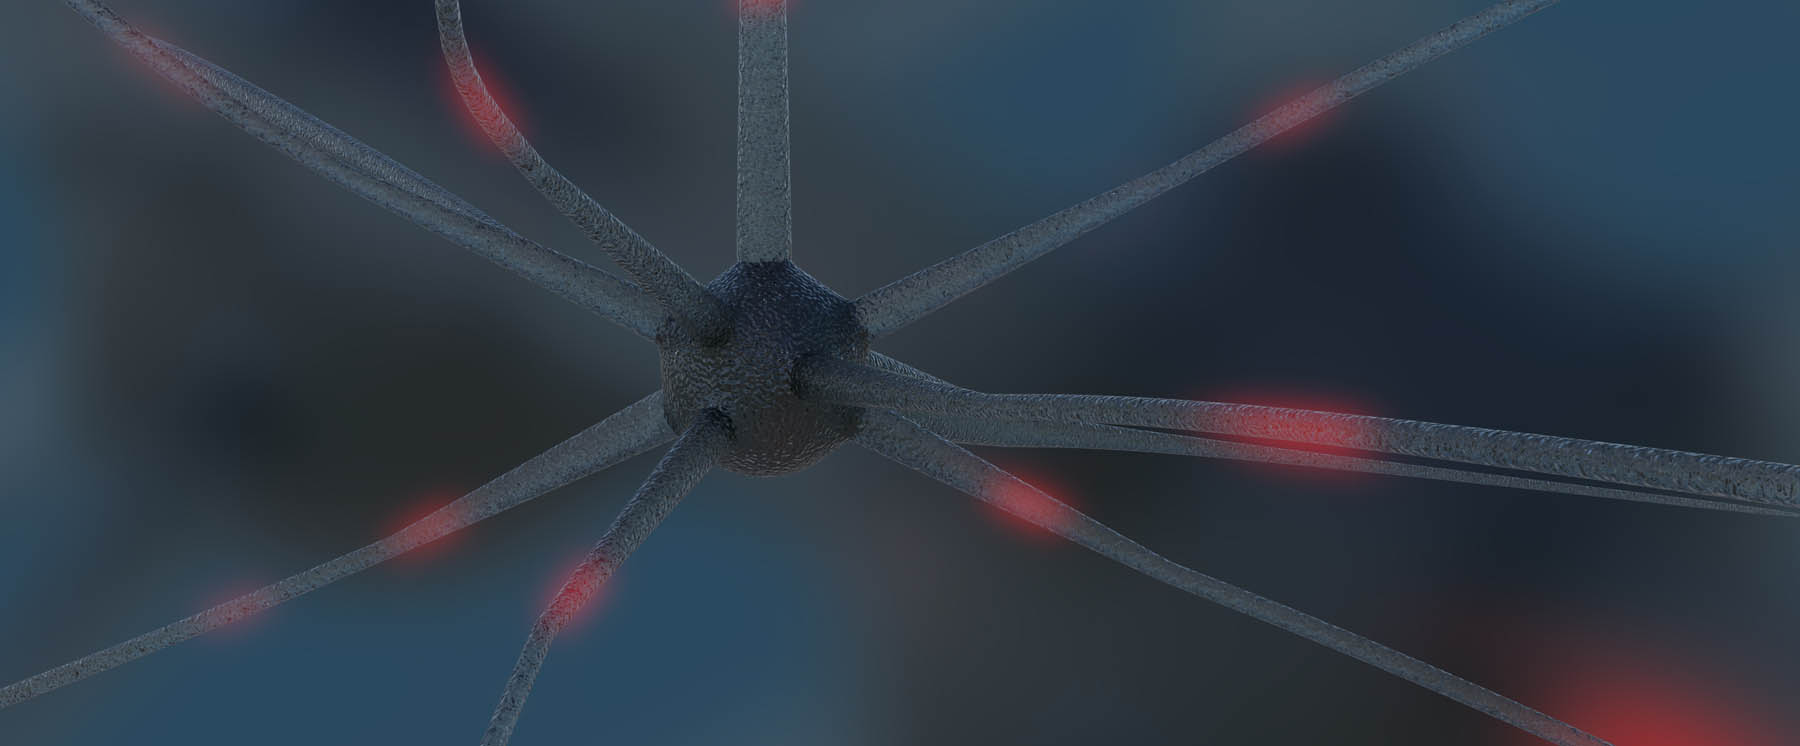
\includegraphics[width=\textwidth]{figures/neurodata-research.jpg}
\small \textit{Image courtesy of \href{https://www.nwb.org/}{www.nwb.org}}
\end{staticcontents*}


\begin{staticcontents*}{frameS-1b}
\vspace{-5cm}
\hspace{1.4cm}
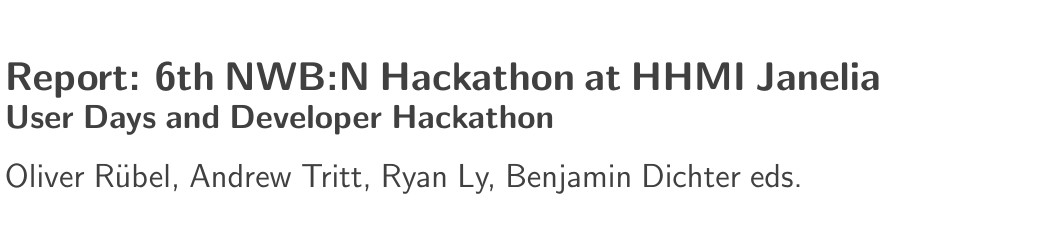
\begin{tikzpicture}
\draw(0,0) node [fill=white, text width=12cm, inner sep=3mm, opacity=0.75]{
\large\sffamily 
%\LARGE\textbf{Report}\\
\Large\textbf{Report: 6th NWB:N Hackathon at HHMI Janelia} \\
\large\textbf{User Days and Developer Hackathon} \\ 
\vspace{0.25cm}
\large Oliver R\"ubel, Andrew Tritt, Ryan Ly, Benjamin Dichter eds. \\
\vspace{0.1cm}
};
\end{tikzpicture}
\end{staticcontents*}

\small


%%%%%%%%%%%%%%%%%%%%%%%%%%%%
% Table of contents
%%%%%%%%%%%%%%%%%%%%%%%%%%%%
%\renewcommand{\baselinestretch}{0.75}\normalsize
\tableofcontents
%\renewcommand{\baselinestretch}{1.0}\normalsize

%%%%%%%%%%%%%%%%%%%%%%%%%%%%
%  Logos on first page
%%%%%%%%%%%%%%%%%%%%%%%%%%%%
\begin{figure}[b!]
%\vspace{-0.2cm}
\vspace{0.3cm}

\includegraphics[width=0.42\textwidth,right]{figures/nwb_n_logo.png} \vspace{0.1cm} \\
\vspace{0.3cm}

\includegraphics[width=0.42\textwidth,right]{figures/kavli_logo.png} \\
\vspace{0.3cm}

\includegraphics[width=0.42\textwidth,right]{figures/lbnl_logo.jpg} \\
%\vspace{0.3cm}

\includegraphics[width=0.42\textwidth,right]{figures/hhmi_logo.png}
\end{figure}


\clearpage


%%%%%%%%%%%%%%%%%%%%%%%%%%%%%
%  User Days Participants
%%%%%%%%%%%%%%%%%%%%%%%%%%%%%%
\begin{staticcontents*}{frameS-2a}
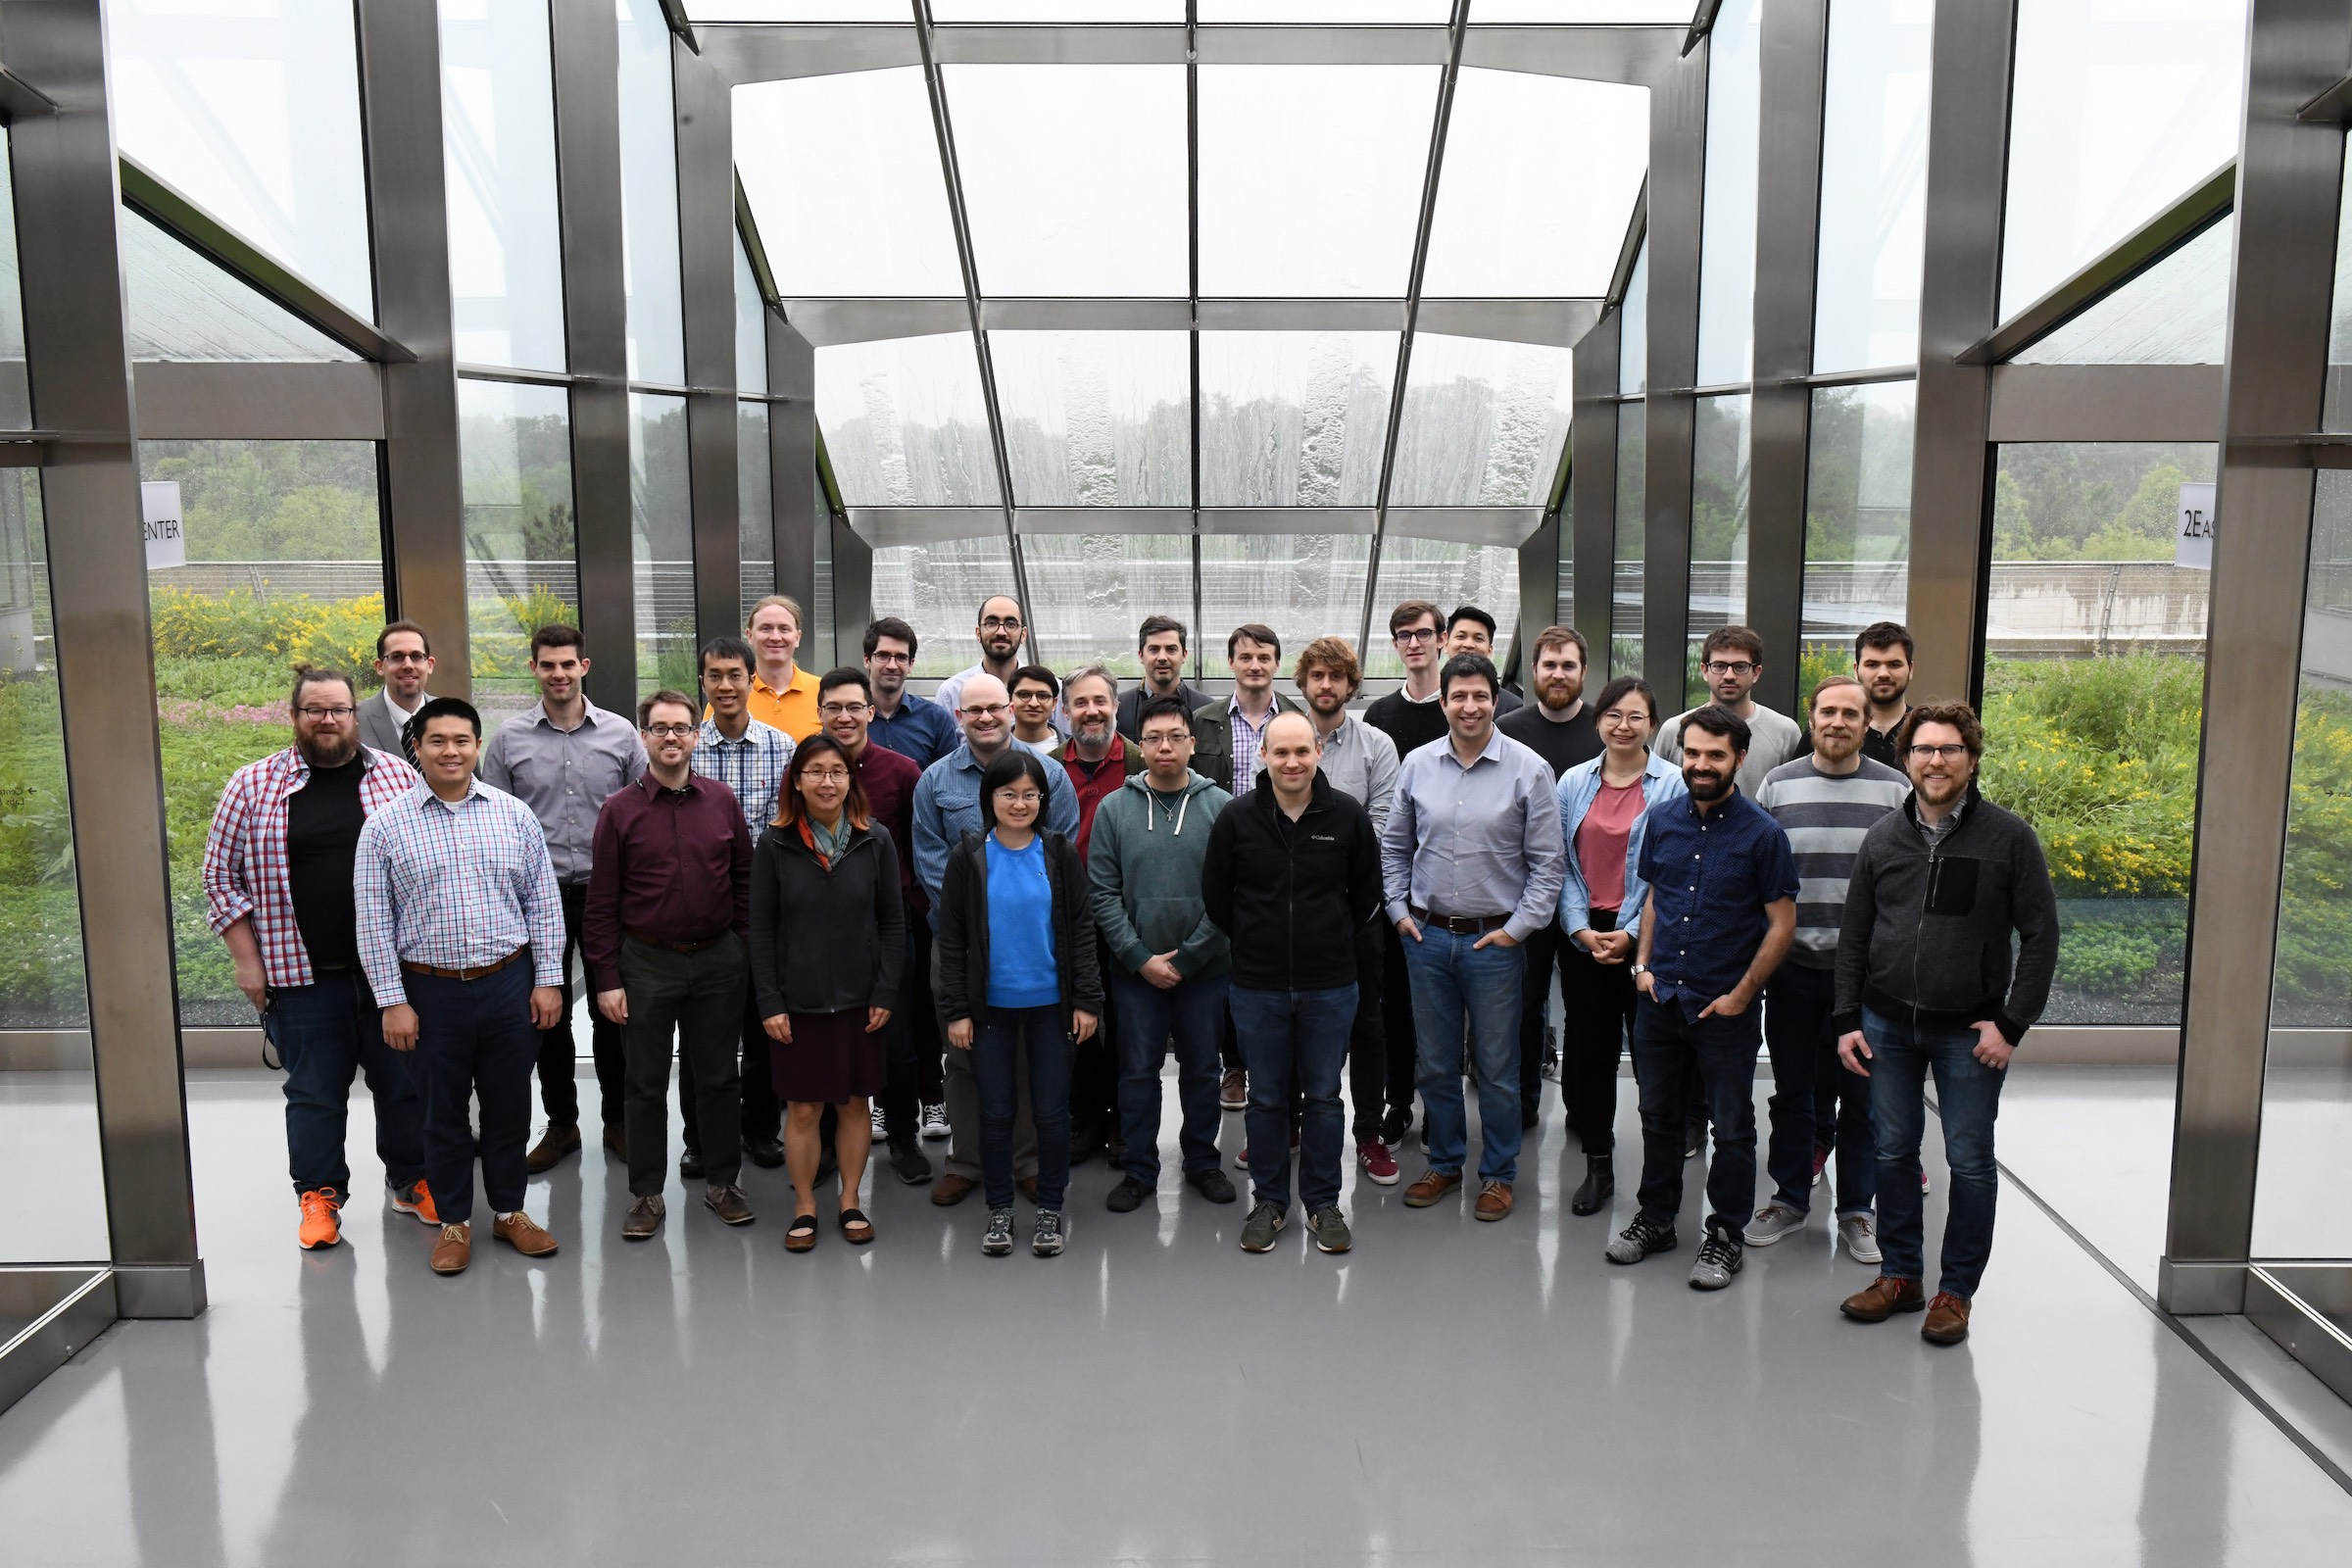
\includegraphics[width=\textwidth]{figures/user_days_group_photo_small.jpg}
Participants of the NWB:N User Days, May 13-14, 2019.
\small \textit{Photo by Matt Staley, HHMI Janelia}
\end{staticcontents*}

\section{Participants -- NWB:N User Days}
\label{sec:userparticipants}

\begin{multicols}{2}
\begin{enumerate}[leftmargin=*]
\setlength\itemsep{0cm}
\item Vyassa Baratham (University of California, Berkeley / Lawrence Berkeley National Laboratory)
\item Jim Berg (Allen Institute for Brain Science)
\item Zac Bowen (University of Maryland Biophysics)
\item Thomas Braun (byte physics)
\item Nand Chandravadia (Cedars-Sinai)
\item Nathan Clack (Vidrio Technologies LLC)
\item Tom Davidson (HHMI/University of California, San Francisco (Frank Lab))
\item Benjamin Dichter (Lawrence Berkeley National Laboratory / Stanford)
\item Nile Graddis (Allen Institute for Brain Science)
\item Michael Grauer (Kitware, Inc.)
\item Roman Huszar (Neuroscience Institute, NYU Langone Health (Buzsaki Lab))
\item Donghe  Kang (The Ohio State University)
\item Adam Kepecs (Cold Spring Harbor Lab)
\item Seth Koehler (Decibel)
\item Andrew Landau (Harvard Medical School)
\item Jessie Liu (University of California, San Francisco  (Chang Lab))
\item Ryan Ly (Lawrence Berkeley National Laboratory)
\item Lydia Ng (Allen Institute for Brain Science)
\item Thinh Nguyen (Vathes LLC)
\item Lawrence Niu (Vidrio Technologies LLC)
\item Peter Petersen (New York University)
\item James Roach (Cold Spring Harbor Lab)
\item Oliver R\"ubel (Lawrence Berkeley National Laboratory)
\item Kelson Shilling-Scrivo (University of Maryland)
\item Matthew Sit (Lawrence Berkeley National Laboratory (Bouchard Lab))
\item Andrew Tritt (Lawrence Berkeley National Laboratory)
\item Jochen Weber (Columbia University)
\item Oscar Woolnough (University of Texas Health Science Center at Houston)
\item Michael Wulf (Cold Spring Harbor Laboratory (Kepecs Lab)
\item Lingling Yang (University of Minnesota)
\item Dimitri Yatsenko (Vathes LLC)
\end{enumerate}
\end{multicols}
\clearpage

%%%%%%%%%%%%%%%%%%%%%%%%%%%%%
%  Developer Days Participants
%%%%%%%%%%%%%%%%%%%%%%%%%%%%%%
\begin{staticcontents*}{frameS-3a}
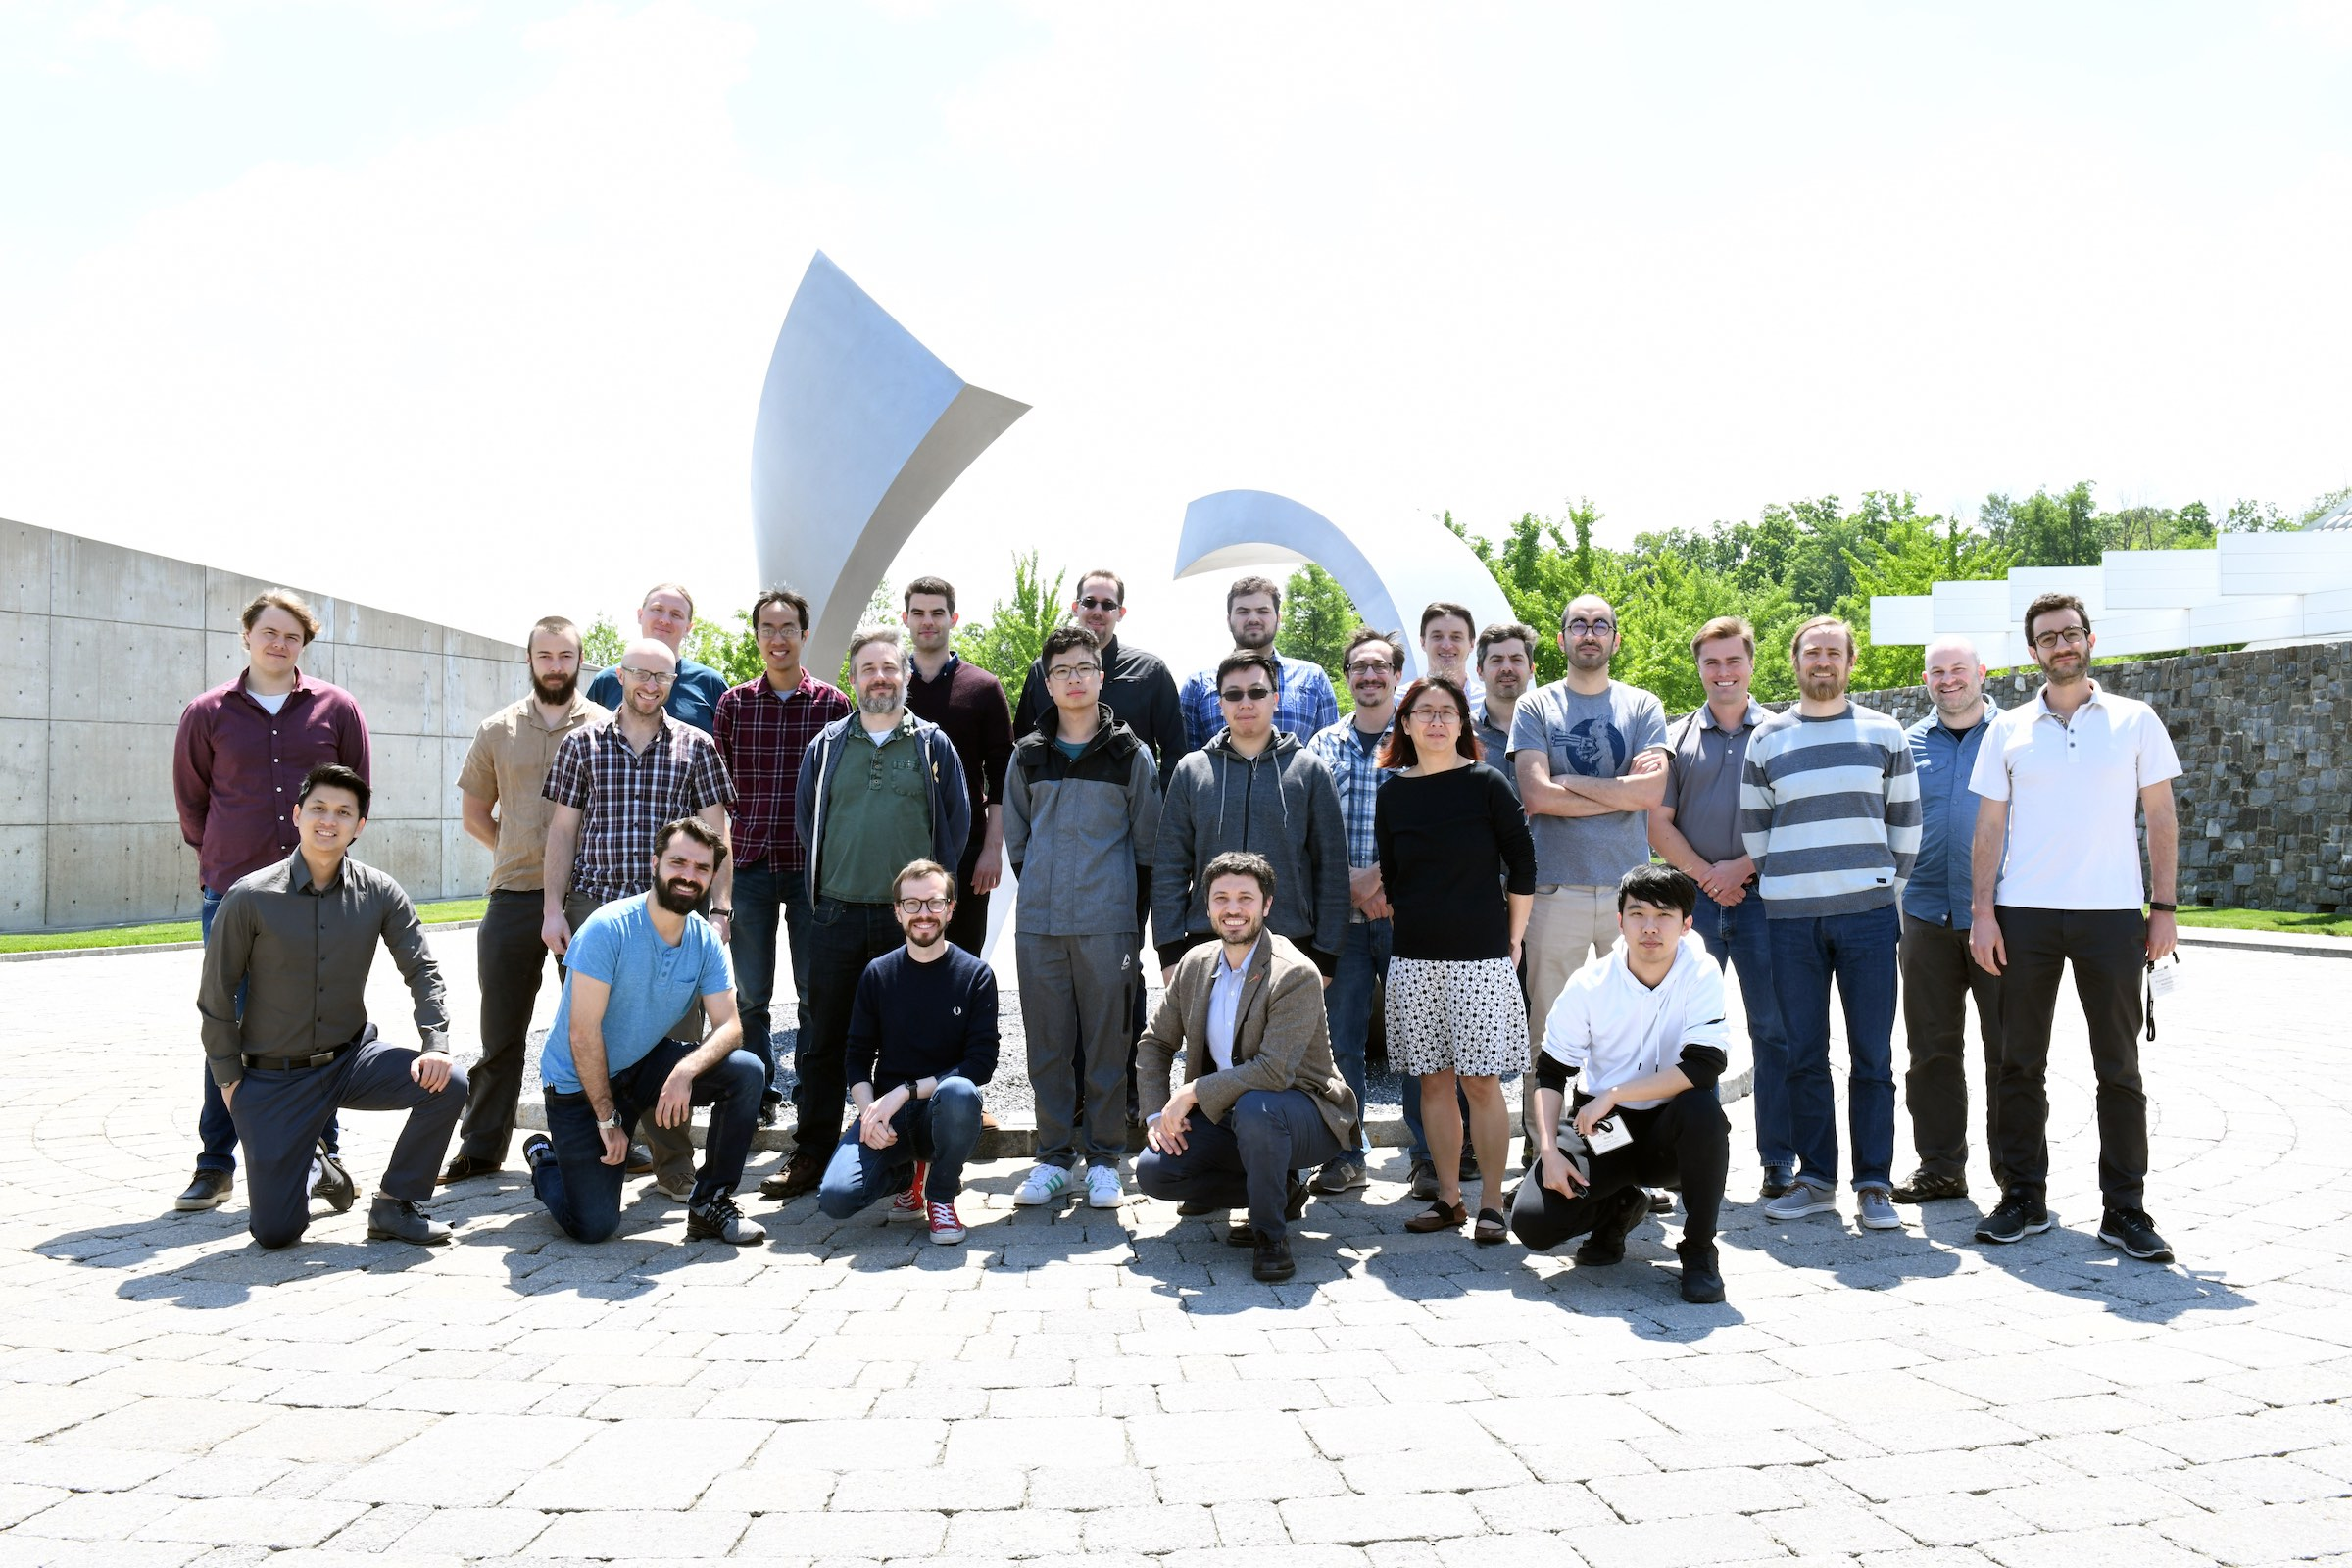
\includegraphics[width=\textwidth]{figures/developer_days_group_photo_small.jpg}
Participants of the NWB:N Developer Days, May 15-16, 2019.
\small \textit{Photo by Matt Staley, HHMI Janelia}
\end{staticcontents*}

\section{Participants -- NWB:N Developer Days}
\label{sec:devparticipants}

\begin{multicols}{2}
\begin{enumerate}[leftmargin=*]
\setlength\itemsep{0cm}
\item Thomas Braun (byte physics)
\item Nicholas Cain (Allen Institute for Brain Science)
\item Nathan Clack (Vidrio Technologies LLC)
\item Tom Davidson (HHMI/University of California, San Francisco (Frank Lab))
\item Benjamin Dichter (Lawrence Berkeley National Laboratory / Stanford)
\item Matthew Earnshaw (University College London)
\item Mohammad Hossein Eybposh (University of North Carolina at Chapel Hill)
\item Jean-Christophe Fillion-Robin (Kitware inc.)
\item Andrea Giovannucci (University of North Carolina at Chapel Hill)
\item Nile Graddis (Allen Institute for Brain Science)
\item Michael Grauer (Kitware, Inc.)
\item Donghe Kang (The Ohio State University)
\item Christian Kellner (G-Node / Red Hat)
\item Mikkel Lepperød (University of Oslo)
\item Ryan Ly (Lawrence Berkeley National Laboratory)
\item Matt McCormick (Kitware Inc.)
\item Konstantinos Nasiotis (Montreal Neurological Institute)
\item Lydia Ng (Allen Institute for Brain Science)
\item Thinh Nguyen (Vathes LLC)
\item Lawrence Niu (Vidrio Technologies LLC)
\item Oliver R\"ubel (Lawrence Berkeley National Laboratory)
\item Will Schroeder (Kitware, Inc.)
\item Andrew Tritt (Lawrence Berkeley National Laboratory)
\item Zhengjia Wang (Baylor College of Medicine/Rice University)
\item Dimitri Yatsenko (Vathes LLC)
\end{enumerate}
\end{multicols}
\clearpage

\section{Executive Summary}
\label{sec:es}

\paragraph{Overview:} The \href{https://neurodatawithoutborders.github.io}{Neurodata Without Borders: Neurophysiology} (NWB:N) project is an effort to standardize the description and storage of neurophysiology data and metadata. NWB:N enables data sharing and reuse and reduces the energy barrier to applying data analytics both within and across labs. The hackathon consisted of a two-day User Days event and a two-day Developer Days event with a joint social on the second day to facilitate interaction between users and developers. For the User Days, we invited experts from the neuroscience research community to learn about NWB:N and to work on projects toward adoption of NWB:N for their lab's data sharing and analysis needs. For the Developer Days, we invited developers from the neuroinformatics community to integrate NWB:N with data analysis, visualization, storage, and management tools, as well as to discuss and design new features for NWB:N and build and improve core NWB:N infrastructure. 
\vspace{-0.2cm}
\paragraph{Participants:} 43 users and developers from 29 major labs and research institutions attended the event (see page~\pageref{sec:userparticipants}-\pageref{sec:devparticipants}). The background in programming among participants at the User Days varied greatly, ranging from beginners to experts, whereas participants at the developer days generally had a strong background in programming. Most participants had investigated NWB:N prior to the event, but many were in the early stages of exploration and adoption. See also the~\nameref{sec:regsurv} for details.

\vspace{-0.2cm}
\paragraph{User Days:} The~\nameref{sec:program:userdays} consisted of a combination of training sessions in the morning and open hacking sessions in the afternoon. A breakout room for hacking was provided at all times to allow users to select the training programs most relevant to their projects. During the coding sessions, participants worked on their \nameref{sec:userprojects}, which they had designed and prepared prior to the event. The user projects generally focused on integration of neuroscience data with NWB:N and involved data from a broad range of~\nameref{sec:regsurv:datamod}, including: a) electrophysiology (extracellular recordings, intracellular recordings, and electrocorticography), b) optophysiology (2-photon imaging, fluorescent wide-field images, etc.), c) behavioral data, d) processed data (e.g., from spike sorting), e) neural simulations (using NEURON software), and f) stimulus data. The user projects also included data from a number of different model species, such as mice, rats, monkeys, and humans. %See the \nameref{sec:userprojects} section for a more in-depth overview of the user projects at the hackathon.

\vspace{-0.2cm}
\paragraph{Developer Days:} The~\nameref{sec:program:devdays} focused on open hacking sessions and breakout sessions to facilitate interaction between developers and discussion on shared topics of interest and current developments, e.g., best practices, extensions sharing, ontologies, data management, and data visualization. The \nameref{sec:userprojects} during the developer days focused on integration of NWB:N with data analysis, visualization, storage, and management software, and development and enhancement of core NWB:N technologies. 

\vspace{-0.2cm}
\paragraph{Select Highlights:} During the user days, users worked on the integration of data from 14+ different labs and institutions with NWB:N. Importantly, all participants were able to make substantial progress during the hackathon towards integration of their data with NWB:N.

Several early adopters---e.g., the Allen Institute for Brain Science, the FrankLab (UCSF), and Buzsaki Lab (NYU)---have by now made first sets of NWB:N data files available to the public. Several other labs, e.g., the ChangLab (UCSF), have indicated plans for upcoming data releases in NWB:N 2.0. Given that NWB:N 2.0 was released in January 2019 (i.e., only $\approx3.5$ month before the hackathon), this fast move towards data releases is impressive and also very important to promote broad adoption of NWB:N. To enable users to easily find public NWB:N files, we have added an \href{https://neurodatawithoutborders.github.io/exampledata}{Example Data} page to the NWB:N website. 

A highlight here was the presentation by Tom Davidson in which he described time-based queries and visualization at the FrankLab. Incidentally, the Allen Institute had released data 1 week prior to the hackathon in NWB:N 2.0 and so they tried their tools on that data as well. ``Because the data was in the NWB:N standard, we were able to very quickly and directly apply our tools to the Allen Institute's data without requiring interaction with the Allen team'' said Tom, ``This showed us that the promise of data reuse and common analysis tools is not just a distant vision but because of NWB:N is within our reach.''

During the developer days, we were excited to see substantial progress toward integration of NWB:N with important data analysis tools, including, Brainstorm, CaImAn, RAVE, NWBWidgets, and the NWBExplorer as part of Open Source Brain. To enable users to more easily discover tools that support NWB:N, we created an \href{https://neurodatawithoutborders.github.io/tools}{Analysis and Visualization Tools} page as part of the NWB:N website. Developers also explored the integration of Zarr and ExDir as alternative storage backends for NWB:N as well as compatibility between NWB:N and Nix and NWB:N and the DataJoint data pipeline management system. Developers also created tools to facilitate the import of data from common data acquisition devices and systems. Another main focus area was the development of core NWB:N technologies, e.g, for data query, extensions sharing, and documentation. 

\vspace{-0.2cm}
\paragraph{Future Directions:} As part of the hackathon, participants suggested several areas that would greatly enhance the utilization and adoptability of NWB:N:
\begin{itemize}
  \setlength\itemsep{0cm}
  \item \textbf{Extensions sharing:} The ability to share and use extensions across labs was recognized as a critical need. Formalizing and standardizing this process will be critical. This is part of current ongoing efforts towards development of the \href{https://github.com/nwb-extensions}{NWB:N Extension Catalog}.
  \item \textbf{Controlled Vocabularies and Ontologies:} The ability to associate controlled terms  (e.g., enumerations) and complex ontologies with NWB:N data fields was recognized as a central need. This is already on the roadmap for NWB:N development as part of ongoing \href{https://braininitiative.nih.gov/funded-awards/nwbn-data-standard-and-software-ecosystem-neurophysiology}{NIH project} and we used the hackathon to interview participants and gather use-cases for the \href{https://github.com/NeurodataWithoutBorders/ontology-project}{NWB:N ontologies project.}
  \item \textbf{Tools for visualization and analysis:} Tools for exploration and visualization of NWB:N was recognized as a general need. This was an active focus of the Developer Days and continues to be a critical thrust area in our outreach activities. 
  \item \textbf{Data search and query:} Advanced tools for search, discovery, and query of NWB:N data are needed to facilitate advanced data analytics. This was also the topic of projects at the Developer Days but we need to expand our efforts in this area as part of future proposals. 
  \item \textbf{Integration with Data Management:} The need for tools to manage large collections of NWB:N files and to facilitate integration of NWB:N with data management tools (e.g., LIMS or DataJoint) was recognized as a common need. While initial efforts in this area are underway, this is a critical area that should be the focus of future proposals. 
  \item \textbf{Documentation, Tutorials, and Standard Import:} While we have made substantial progress over the last 2 years in creating documentation and tutorials, this area requires continued effort and improvement. In particular the need for additional high- and entry-level documentation was recognized and was also the focus of several Developer Days projects. 
\end{itemize}

\vspace{-0.2cm}
\paragraph{Conclusion:}
By the end of the hackathon, the vast majority of attendees had accomplished many of their goals, and several were well on their way to having NWB:N fulfill their labs needs. All attendees indicated an enthusiasm for the current software and were impressed with the (relative) ease of use given the generality. Overall, the hackathon was a great success. See also the \nameref{sec:exitsurv} for further details.

Based on discussions at the hackathon, we plan to have another hackathon in a year for both users and developers. In addition we are also hoping to have a developer-focused hackathon in November to facilitate continued development and close interaction between the developers, to discuss design and strategy, and engage more closely with user projects and use cases. 

%\clearpage
\subsection{Organization}

The meeting was organized by Oliver R\"ubel (organizer), Benjamin Dichter (co-organizer), and Karel Svoboda (site chair) with logistics and organizational support by Janine Stevens (HHMI Janelia), AV support by Matt Staley (HHMI Janelia), and travel support by Stephanie Albin (Kavli Foundation). Travel support was provided by the Kavli Foundation.  Housing, food and other meeting resources were sponsored by HHMI Janelia. 

\begin{figure*}[h!]
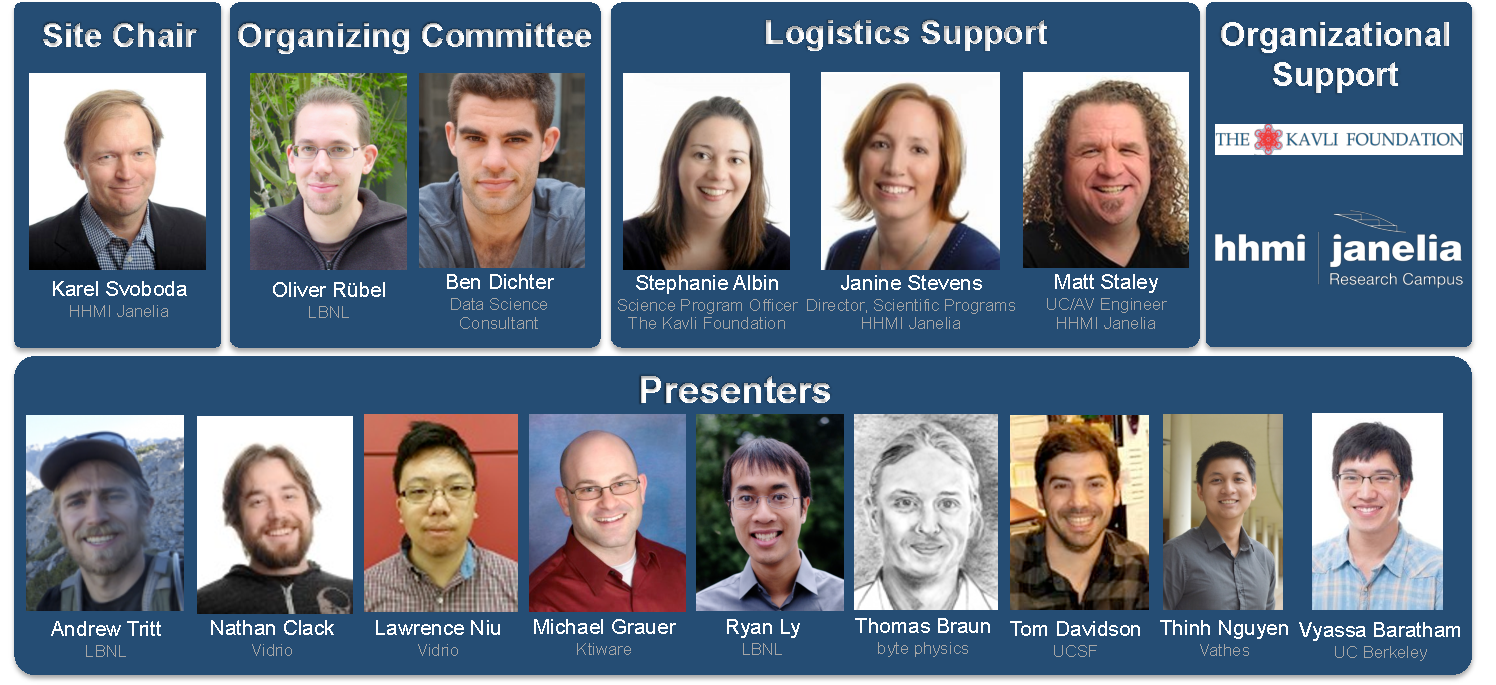
\includegraphics[width=15.5cm]{figures/organization_and_presenters.pdf}
\end{figure*}


\subsection{Suggestions for Specific Developments}
\label{sec:es:dev}

In addition to the more high-level direction for future development discussed in the \nameref{sec:es}, we here describe additional, specific developments that were suggested by participants at the hackathon. 

\begin{itemize}
 \setlength\itemsep{0cm}
 \item Easily query within and across NWB:N files for particular data. For example, show me the recorded voltage traces after stimulus X for animals with manipulation Y that were tested between D1 and D2.
 \item Improve the tutorials to cater toward researchers with less programming experience. Users also mentioned that it would be very useful to include more graphics that depict how data is stored and have working boilerplate code where the user just needs to change a few variables to accommodate their data. 
 \item Develop better tutorials to the MatNWB API, and add more convenience functions like in the PyNWB API.
 \item Add ability to define time points within a trial and re-reference timestamps and time series data relative to those time points. For example, users want to easily represent voltage traces aligned to reward time, across trials.
 %\item Add ability to store trialized data, e.g. time series data that has already been segmented by trials, %without having to supply the full time series data, which is not always available.
 \item Add ability to organize raw acquisition data rather than having them all in the same group. This is currently possible for processed data but not acquisition data.
 \item Create a plotting gallery for different neurodata types.
 \item Improve validation of NWB:N files.  
 \item Add ability to dump state of PyNWB/MatNWB during read/write for better debugging.
\end{itemize}


\clearpage
\section{Registration Survey}
\label{sec:regsurv}

As part of the registration we asked all participants about: which 1) software tools and 2) programming languages they are using to interact with their data as well as 3) which data modalities they are using. The questions where posed as multiple-choice questions with the option for users to provide custom other responses. 34 users registered for the User Days, of which 31 attended the User Days. 26 developers registered, of which 25 attended the Developer Days. In total, 45 unique people responded to the survey, i.e., some folks attended and responded to the survey for both the User- and Developer days. 

\vspace{-0.2cm}
\subsection{Software Tools}

{\setlength{\parindent}{0cm}
\textbf{Survey Question}: Which software tools are you using to interact with your data? \\
\textbf{Response Options:}: 1) PyNWB, 2) MatNWB, 3) Other (user provides text) \\
\textbf{Number of User Days Responses:} 34 of 34 \\ 
\textbf{Number of Developer Days Responses:} 25 of 25 
}

\begin{figure*}[h!]
   \begin{subfigure}[b]{0.49\textwidth}
        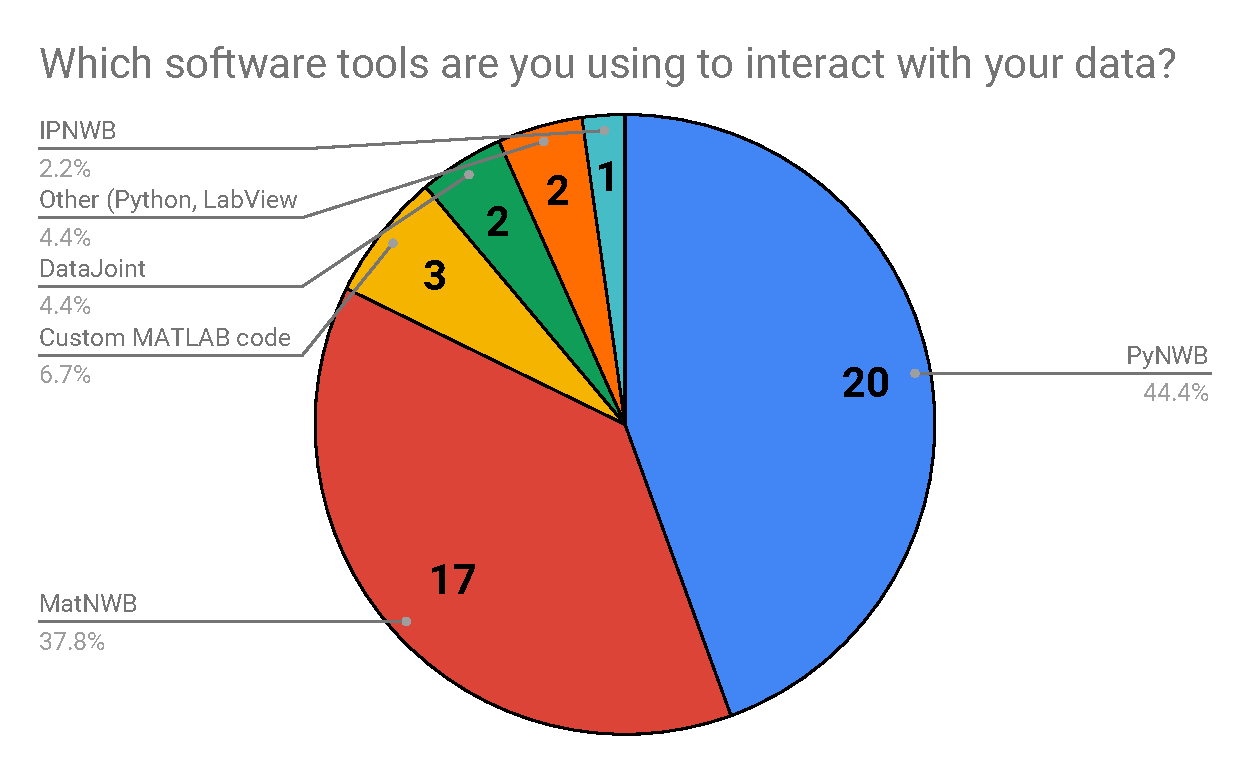
\includegraphics[width=\textwidth]{figures/users_nwb_software_presurvey.pdf}
        \caption{NWB:N User Days}
    \end{subfigure}
    \begin{subfigure}[b]{0.49\textwidth}
        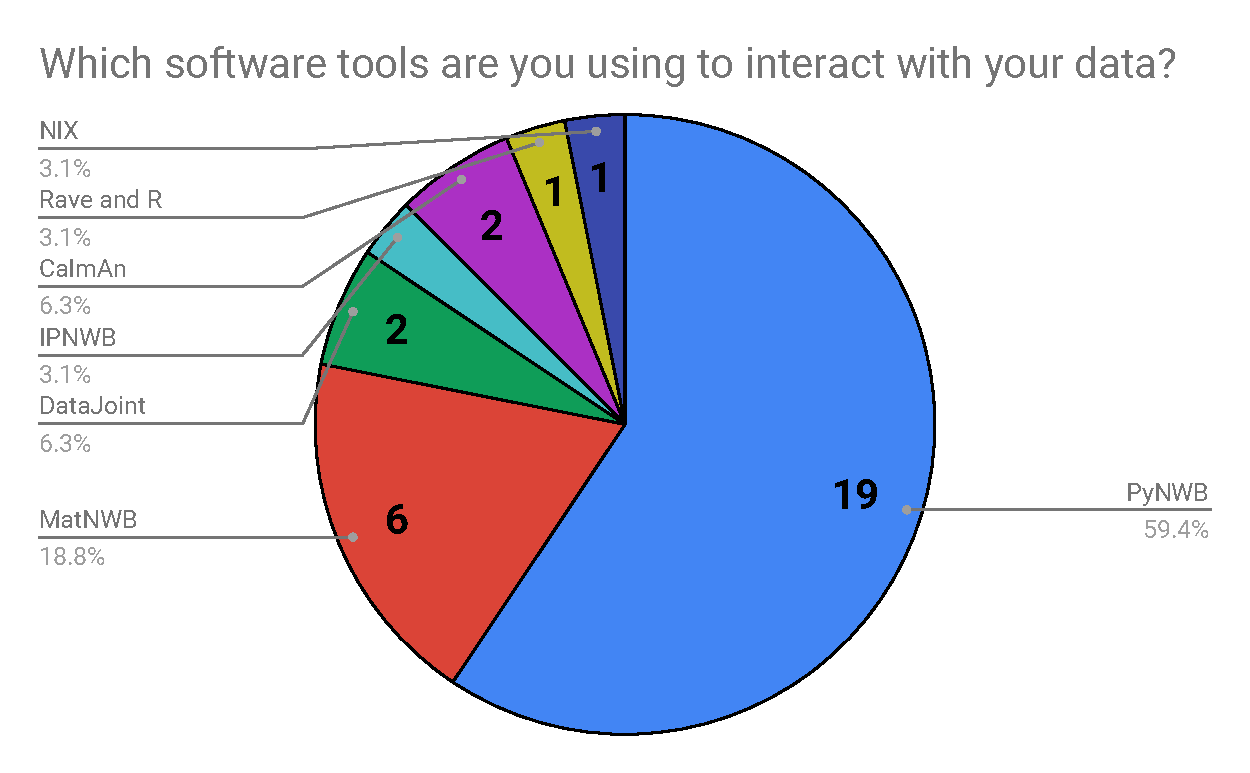
\includegraphics[width=\textwidth]{figures/developers_nwb_software_presurvey.pdf}
        \caption{NWB:N Developer Days}
    \end{subfigure}
    \caption{Registration survey responses for the user days (a) and developer days (b) on: ``Which software tools are you using to interact with your data?''}
\end{figure*}

\vspace{-0.2cm}
\subsection{Programming Languages}

{\setlength{\parindent}{0cm}
\textbf{Survey Question}: Which programming languages are you using to interact with your data? \\
\textbf{Response Options:}: 1) Python, 2) Matlab, 3) C/C++, 4) Julia, 5) Java, 6) Other (user provides text) \\
\textbf{Number of User Days Responses:} 34 of 34 \\ 
\textbf{Number of Developer Days Responses:} 25 of 25 
}

\begin{figure*}[h!]
   \begin{subfigure}[b]{0.49\textwidth}
        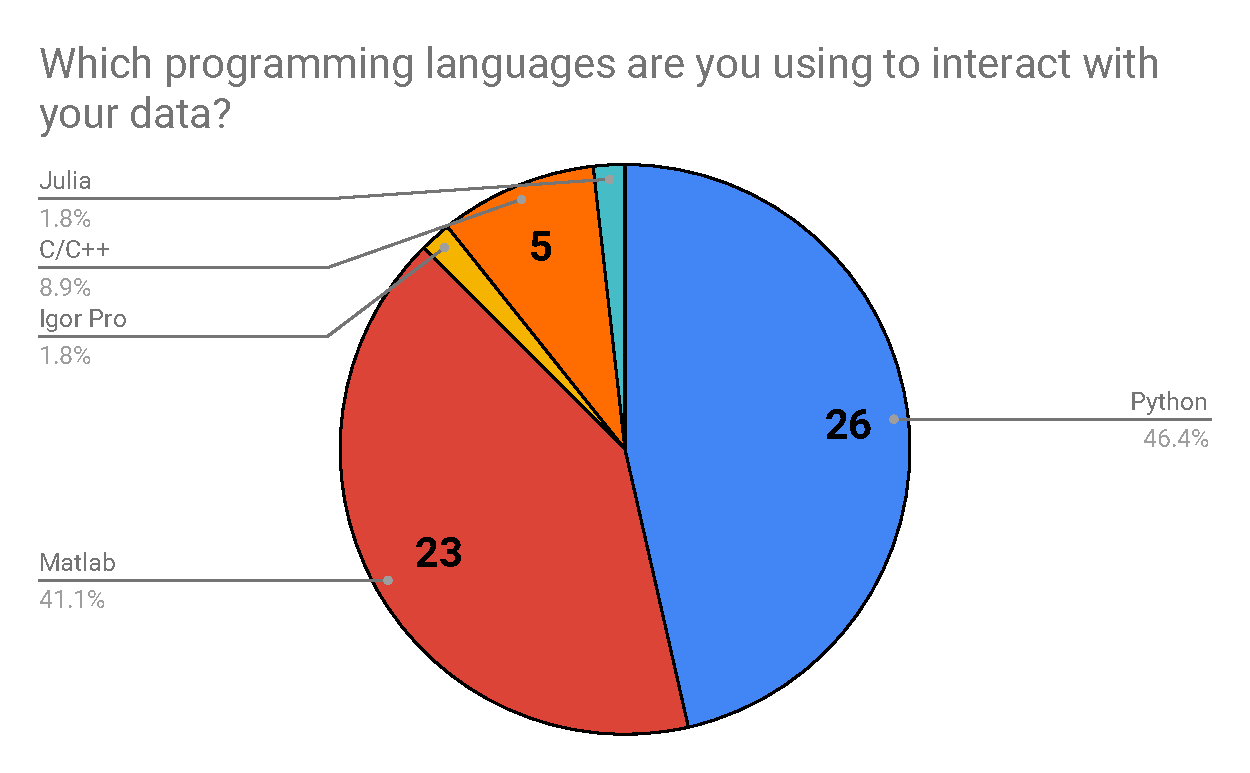
\includegraphics[width=\textwidth]{figures/users_nwb_programlang_presurvey.pdf}
        \caption{NWB:N User Days}
    \end{subfigure}
    \begin{subfigure}[b]{0.49\textwidth}
        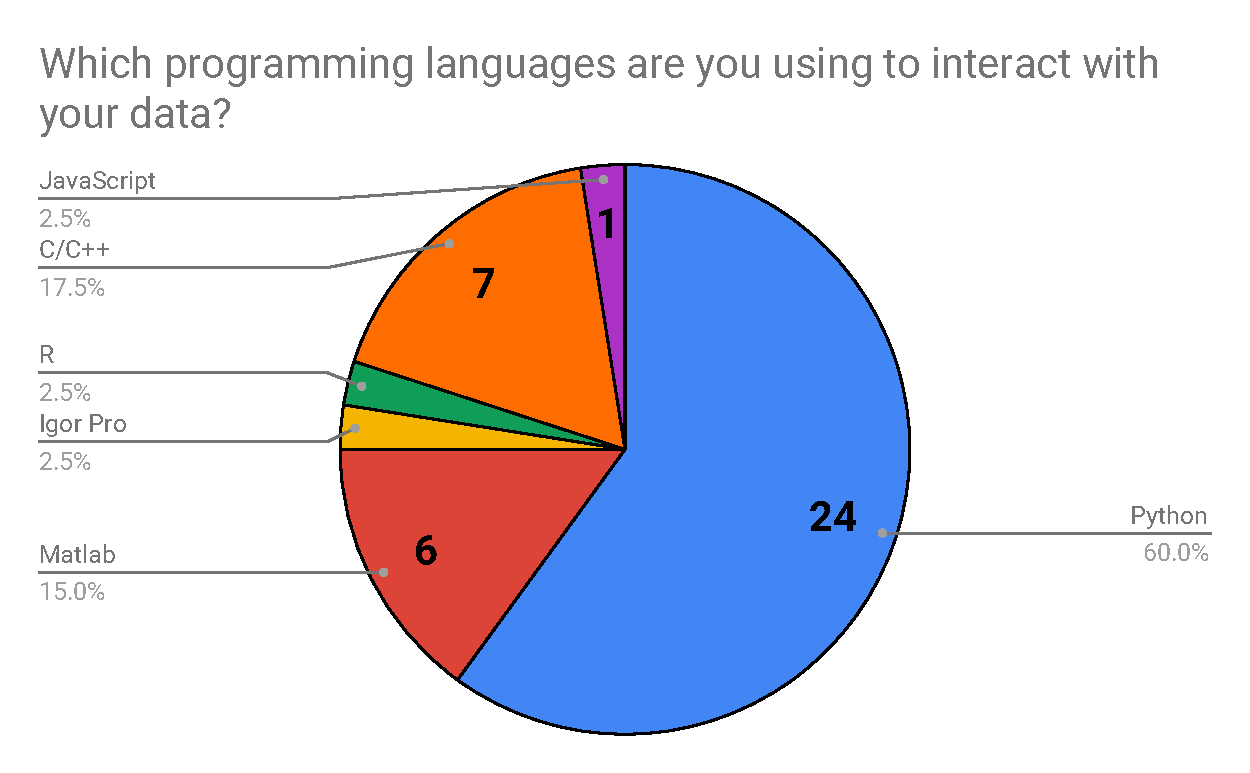
\includegraphics[width=\textwidth]{figures/developers_nwb_programlang_presurvey.pdf}
        \caption{NWB:N Developer Days}
    \end{subfigure}
    \caption{Registration survey responses for the user days (a) and developer days (b) on: ``Which programming languages are you using to interact with your data?''}
\end{figure*}

\subsection{Data Modalities}
\label{sec:regsurv:datamod}

{\setlength{\parindent}{0cm}
\textbf{Survey Question}: Which data modalities are you using? \\
\textbf{Response Options:}: 1) Extracellular ephys, 2) Intracellular ephys, 3) Ca imaging, 4) Behavioral recordings, 5) Other (user provides text) \\
\textbf{Number of User Days Responses:} 28 of 34 \\ 
\textbf{Number of Developer Days Responses:} 22 of 25 
}

\begin{figure*}[h!]
   \begin{subfigure}[b]{0.49\textwidth}
        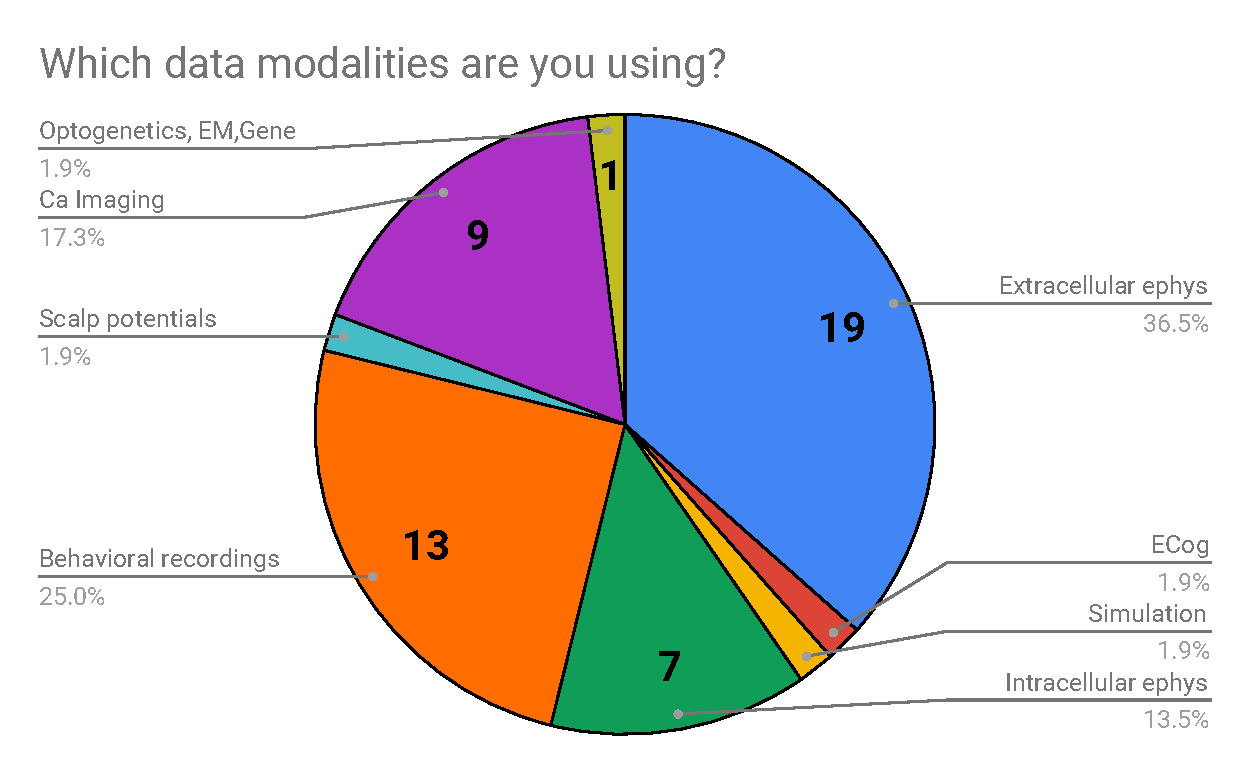
\includegraphics[width=\textwidth]{figures/users_nwb_data_modality_presurvey.pdf}
        \caption{NWB:N User Days}
    \end{subfigure}
    \begin{subfigure}[b]{0.49\textwidth}
        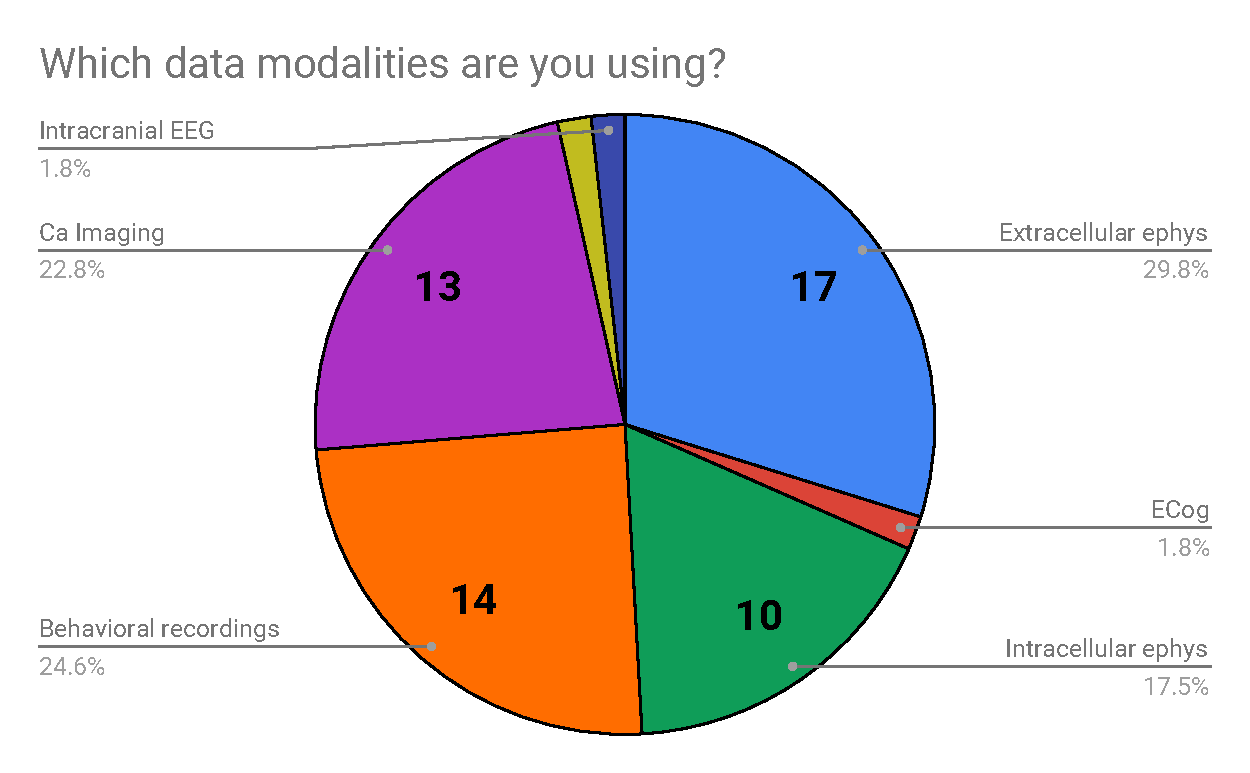
\includegraphics[width=\textwidth]{figures/developers_nwb_data_modality_presurvey.pdf}
        \caption{NWB:N Developer Days}
    \end{subfigure}
    \caption{Registration survey responses for the user days (a) and developer days (b) on: ``Which data modalities are you using?''}
\end{figure*}

%\subsubsection*{Text-based survey questions}
%
%{\setlength{\parindent}{0cm}
%\textbf{Survey Question}: What is your interest in NWB:N? \\
%}
%
%{\color{red} 
%\begin{itemize}
%    \item 
%\end{itemize}
%}
%
%{\setlength{\parindent}{0cm}
%\textbf{Survey Question}: Which projects are you planning to use NWB:N for? \\
%}
%
%{\color{red} Add responses
%\begin{itemize}
%    \item 
%\end{itemize}
%}
%
%{\setlength{\parindent}{0cm}
%\textbf{Survey Question}: How are you using NWB:N? \\
%}
%
%{\color{red} Add responses
%\begin{itemize}
%    \item 
%\end{itemize}
%}
%
%{\setlength{\parindent}{0cm}
%\textbf{Survey Question}: What would you like to achieve at the event? \\
%}
%
%{\color{red} Add responses
%\begin{itemize}
%    \item 
%\end{itemize}
%}



\clearpage
\section{Exit Survey}
\label{sec:exitsurv}

All participants were asked to participate in an exit survey. 15 of the 42 participants (i.e., $~31\%$) submitted responses 
to the survey. 12 of the 15 respondents attended the user days.

\subsection{Hackathon Overall and Testimonials}
\begin{figure*}[h!]
\centering
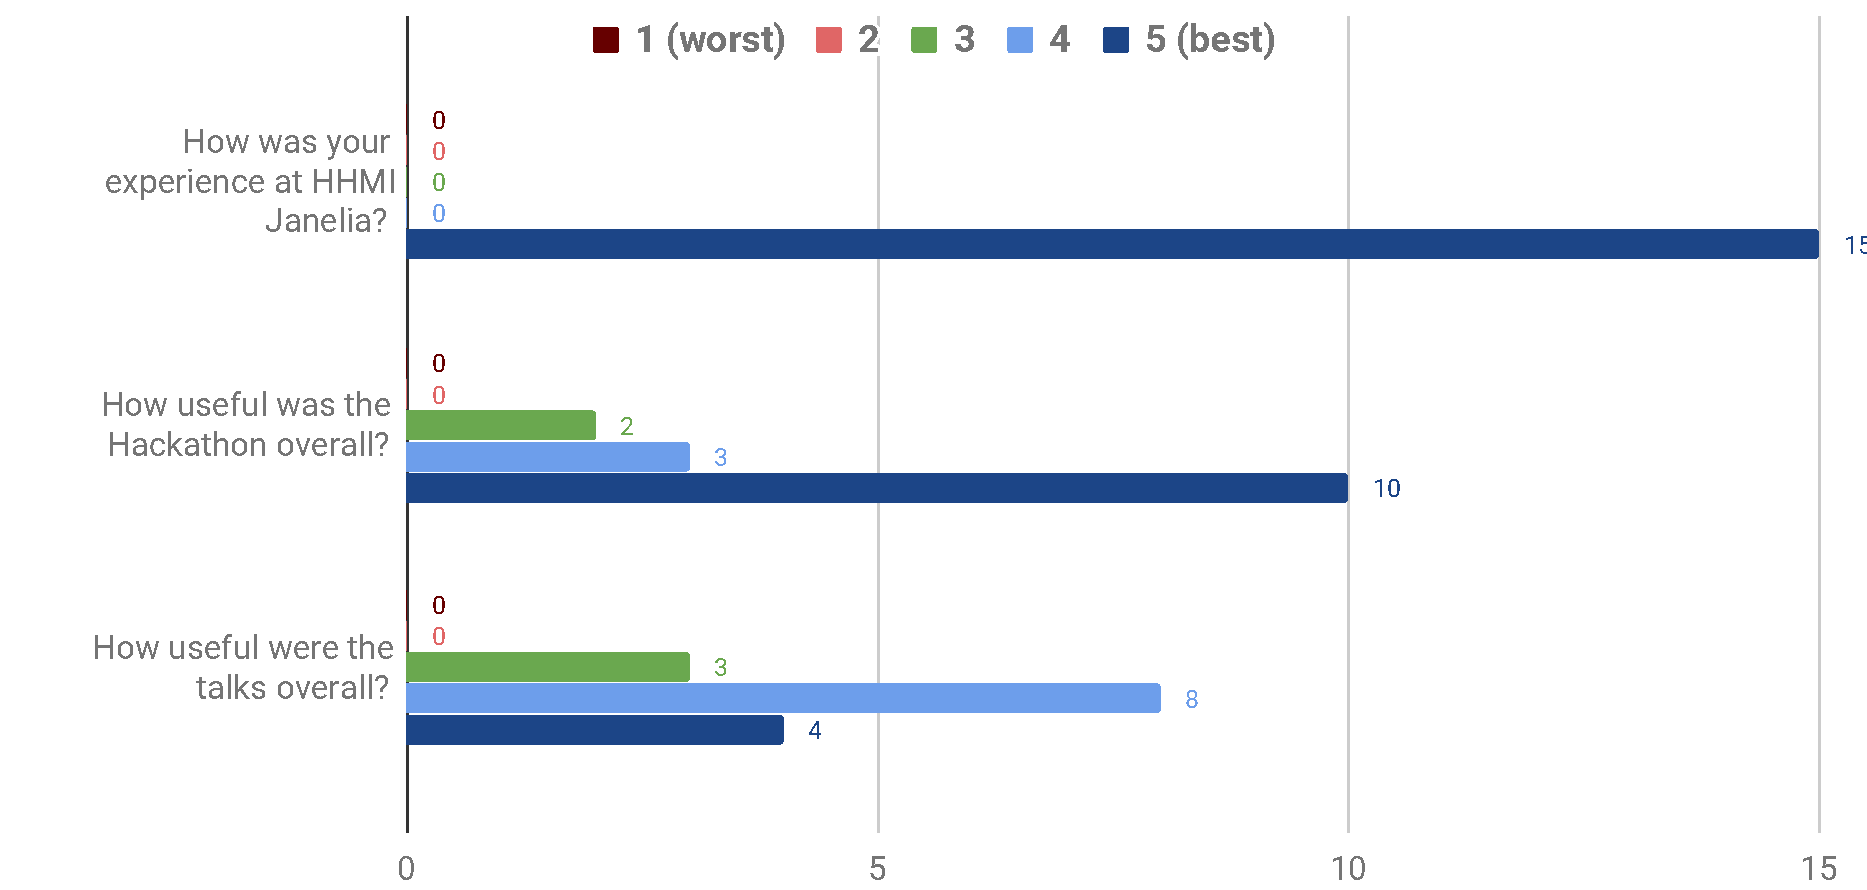
\includegraphics[width=\textwidth]{figures/user_developer_exit_survey_hackathon.pdf}
\end{figure*}

\noindent On a scale of 1 (worst) to 5 (best) the average ratings for the hackathon were excellent, which is also reflected in the testimonials the participants provided:
\begin{itemize}
    \item \textbf{5} : Experience at HHMI Janelia
    \item \textbf{4.5} : Usefulness of the hackathon overall
    \item \textbf{4.1}: Usefulness of the talks overall
\end{itemize}


\subsubsection*{Testimonials}
As part of the exit survey we asked folks whether they would like to provide any testimonials. The exit survey was anonymous, i.e.,
testimonials are also anonymous unless participants submitted them via email. 

\begin{itemize}
    \item The NWB Hackathon User Days was incredibly useful. Well organized, developers were always present and helpful with answering questions. They created an environment of users and developers coming together to help each other, it was refreshing and so conducive to all the good work that has come out of it!
    \item Coming from zero experience with NWB, the hackathon was very useful to have the developers there to aid with questions the whole time. The whole developer team was so receptive to feedback and quick to make changes to make the users experience better. It was nice to connect with other researchers who are facing similar data management issues and trying to move to NWB. The Janelia research campus was a great venue for the event.
    \item The organizers did an awesome job putting together a hackathon that provided (1) a needed refresher and overview, (2) opportunity to ask questions, and (3) space to work on the datasets in the hacking sessions. Overall close to perfect balance. Thank you!!
    \item Michael Grauer (Kitware):  ``I wanted to say thanks and congrats for putting on a fantastic hackathon. Personally I
really enjoyed it, it was super productive for both me and the Kitware team. I think 
this gave the community a lot of cohesion and momentum, which is a great sign for things 
to come.''
\end{itemize}

\clearpage
\subsection{Software}
\begin{figure*}[h!]
\centering
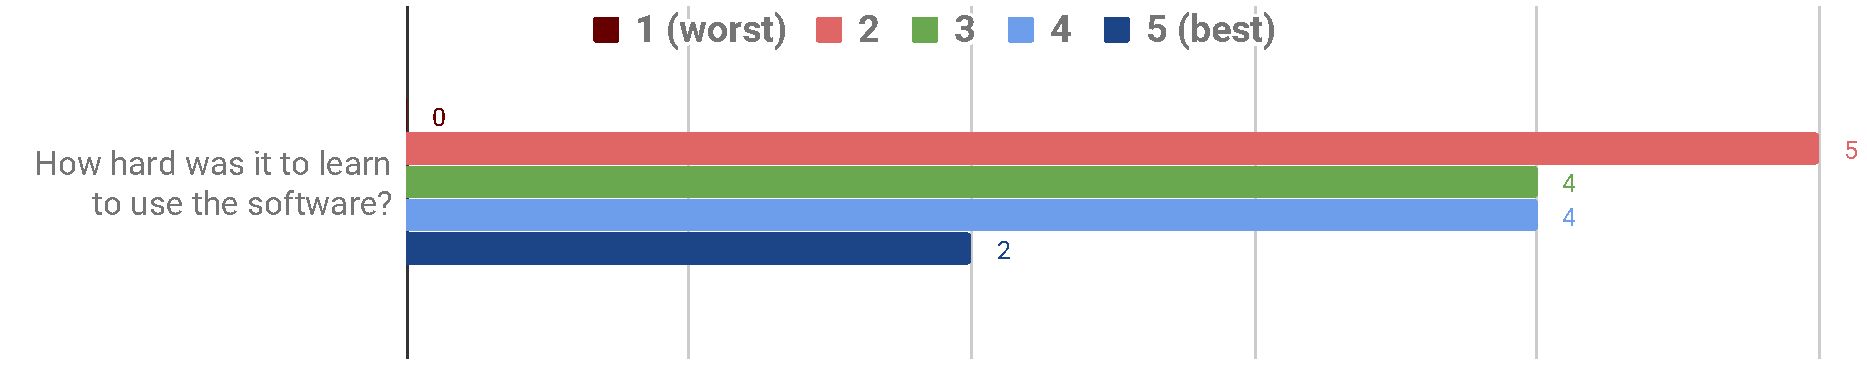
\includegraphics[width=\textwidth]{figures/user_developer_exit_survey_software.pdf}
\end{figure*}

\noindent On a scale of 1 (worst) to 5 (best) the average ratings for how hard it was to learn to use the software was \textbf{3.2}. 

\subsection{Talks and Tutorials}

\begin{figure*}[h!]
\centering
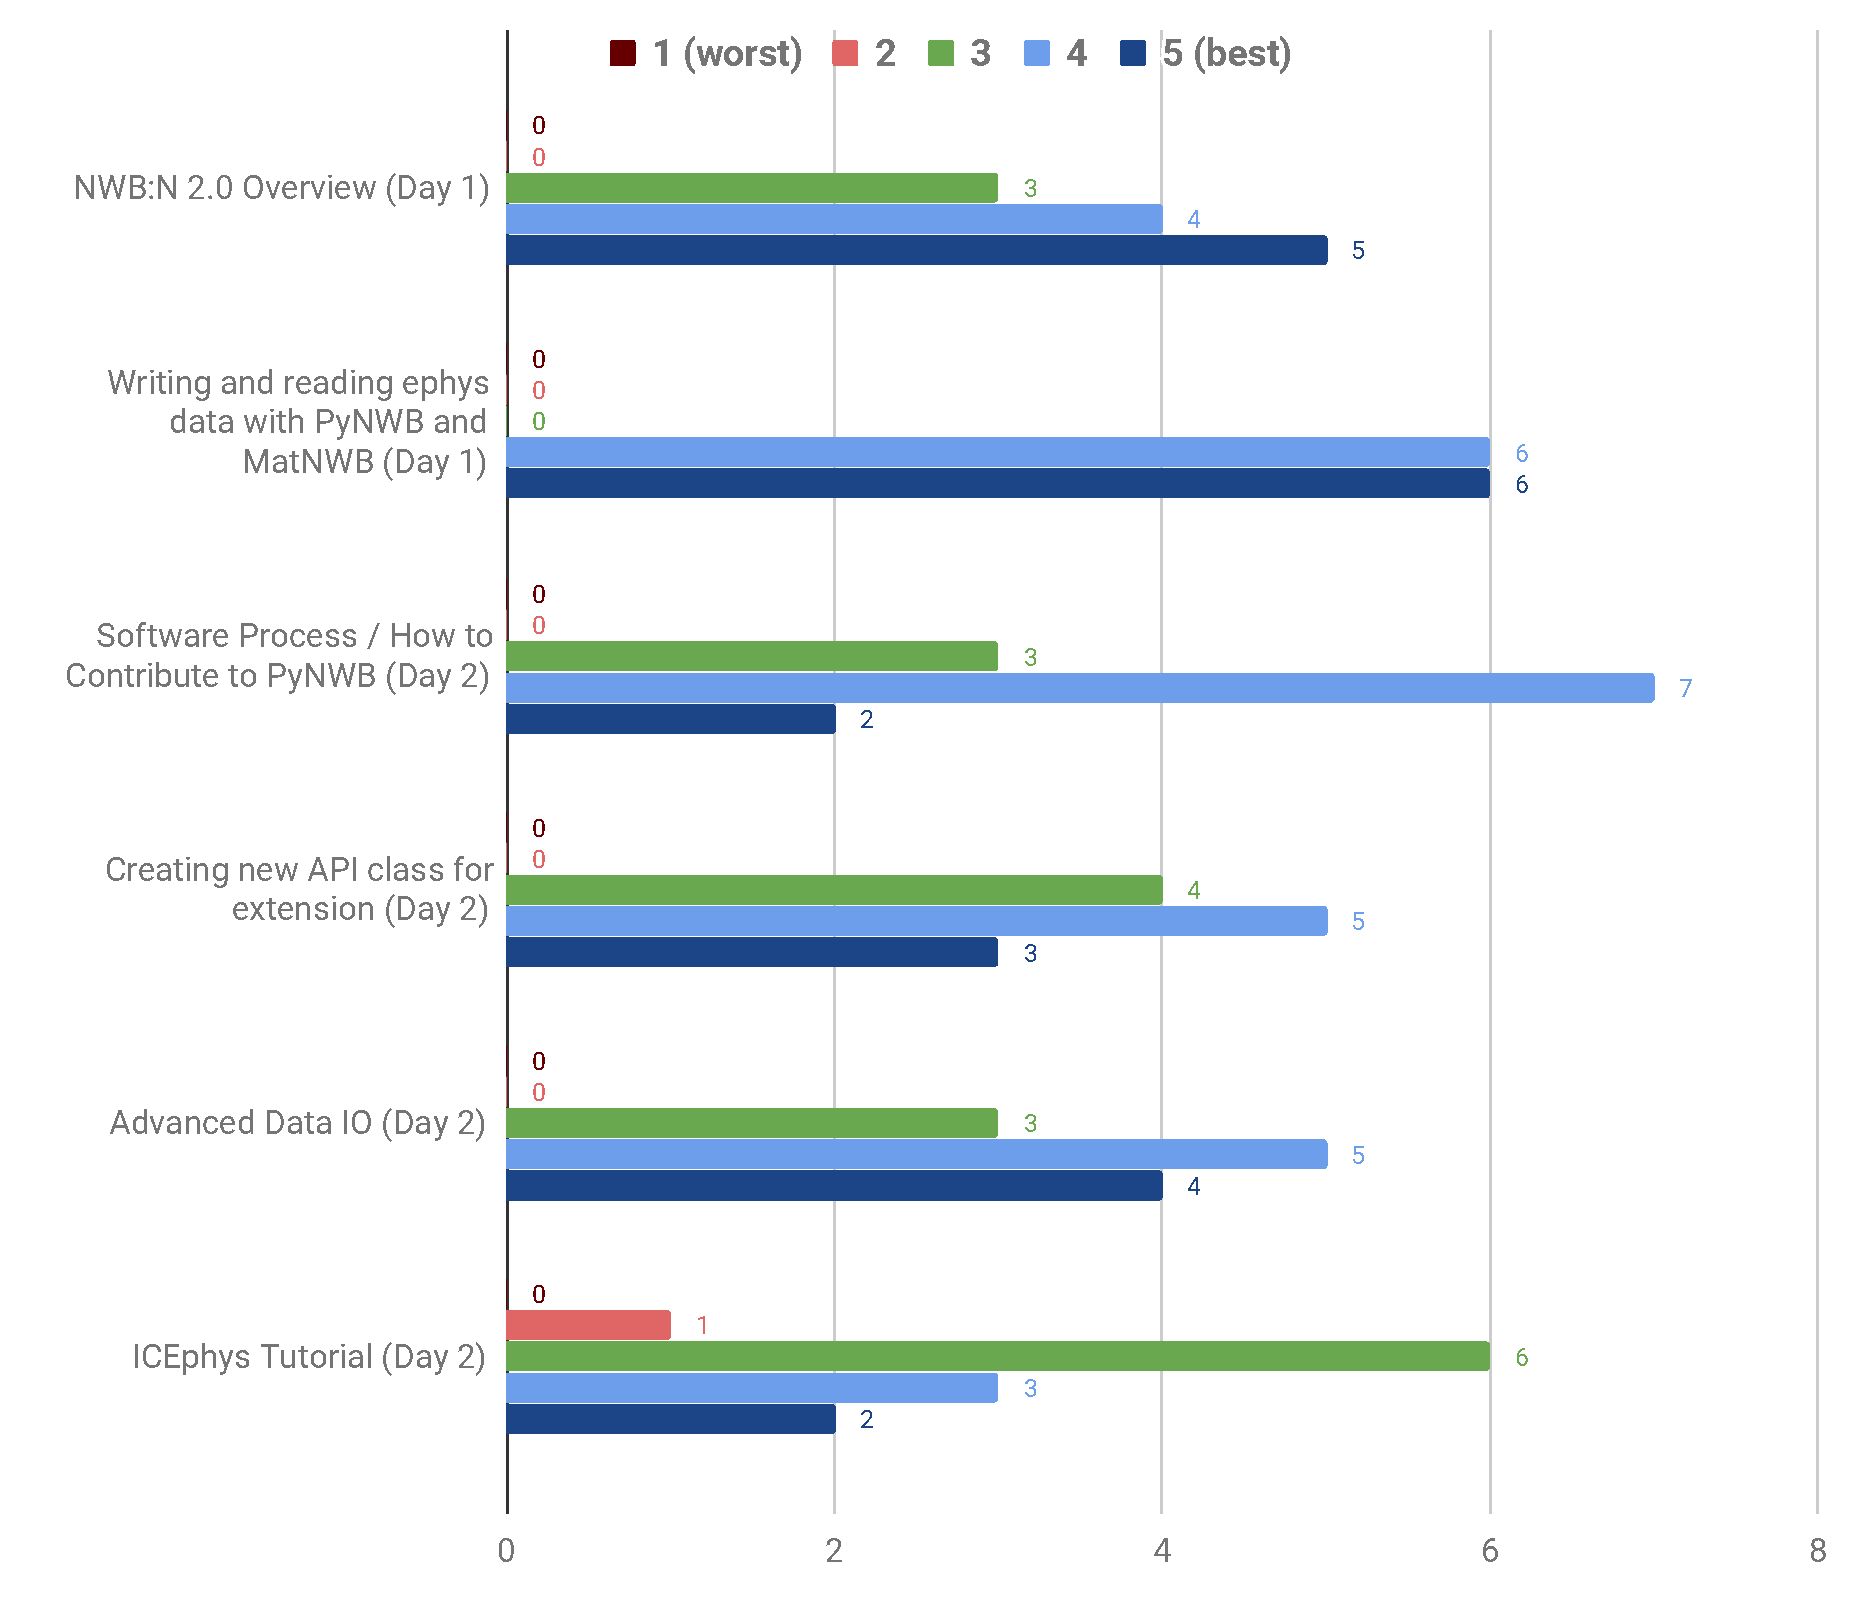
\includegraphics[width=\textwidth]{figures/user_developer_exit_survey_talks.pdf}
\end{figure*}

\noindent Overall the talks were well-received, with average ratings of \textbf{4.2, 4.5, 3.9, 3.9, 4.1,} and \textbf{3.5}, respectively. 

To further improve the ease of on-boarding as folks adopt NWB:N, survey participants suggested the creation of simple, reusable examples. Specific suggestions from the exit survey included:
\begin{itemize}
    \item ``The tutorials provided were very helpful but also have room for improvement (and they have been updated already which is nice). I think it needs to be more clear which aspect of the tutorials are or are not necessary to create a NWB file (i.e. I would start from the most basic bare-bones NWB file and build up from there). I think some generalized examples of how to add in different types of data would go a long way, with detail explaining the intention of each step and why things are stored the way they are. Maybe these exist and I just missed them. It might be too much to ask, but usage examples would be helpful on the docs for each different type (nwb-schema.readthedocs.io).''
    \item ``To simplify people getting started with, especially, their format conversion projects, having a collection of boilerplate codes (that is approved and tested by NWB contributors!) would be super helpful, IMO.''
\end{itemize}

In response to specific user suggestion we have clarified and updated many of the existing online tutorials. We also started a project with the goal to create an \href{https://neurodatawithoutborders.github.io/nwb_hackathons/HCK06_2019_Janelia/projects/Interactive_PyNWB_Course/}{interactive online course for PyNWB}. Improving and expanding documentation and tutorials is an important and perpetual effort. Our goal is to make NWB:N as easy-to-use as possible, and documentation and tutorials are key parts of that. 

\clearpage

\section{Program}
\label{sec:program}

\begin{itemize}
  \item \textbf{Event Website:} \href{https://neurodatawithoutborders.github.io/nwb_hackathons/HCK06\_2019\_Janelia/}{https://neurodatawithoutborders.github.io/nwb\_hackathons/HCK06\_2019\_Janelia/}
  \item \textbf{Dates:} May 13-16, 2019
  \begin{itemize}
     \setlength\itemsep{0cm}
      \item \textbf{User Days:} May 13-14, 2019
      \item \textbf{Developer Days:} May 15-16, 2019
    \end{itemize}
  \item \textbf{Location:}  Location: HHMI Janelia Research Campus, 19700 Helix Dr, Ashburn, VA 20147
  \item \textbf{Slides:} The slides from the talks and tutorials presented at the event are available online at: \\ \href{https://neurodatawithoutborders.github.io/nwb\_hackathons/HCK06\_2019\_Janelia/\#resources}{https://neurodatawithoutborders.github.io/nwb\_hackathons/HCK06\_2019\_Janelia/\#resources}
\end{itemize}


\subsection{User Days Program}
\label{sec:program:userdays}
\begin{figure*}[h!]
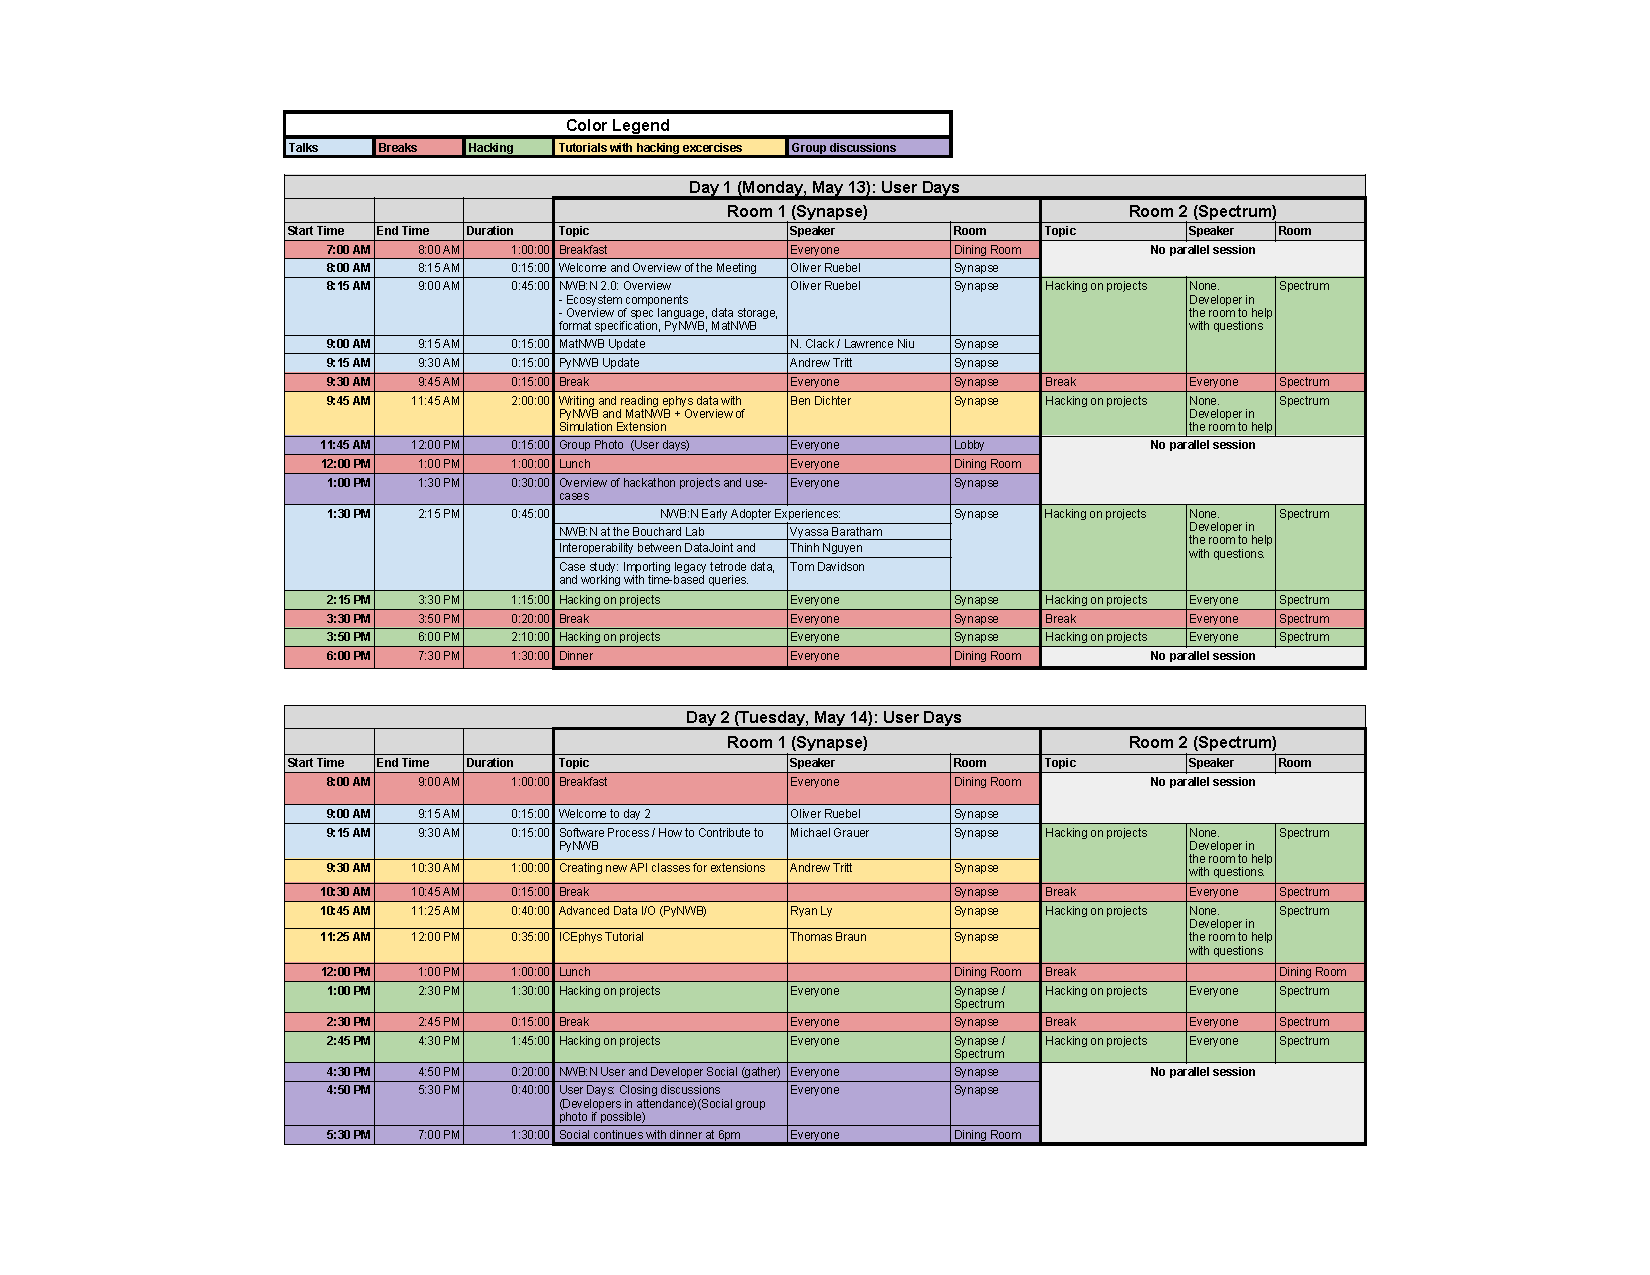
\includegraphics[width=\textwidth]{figures/agenda_user_days.pdf}
\end{figure*}

\clearpage
\subsection{Developer Days Program}
\label{sec:program:devdays}
\begin{figure*}[h!]
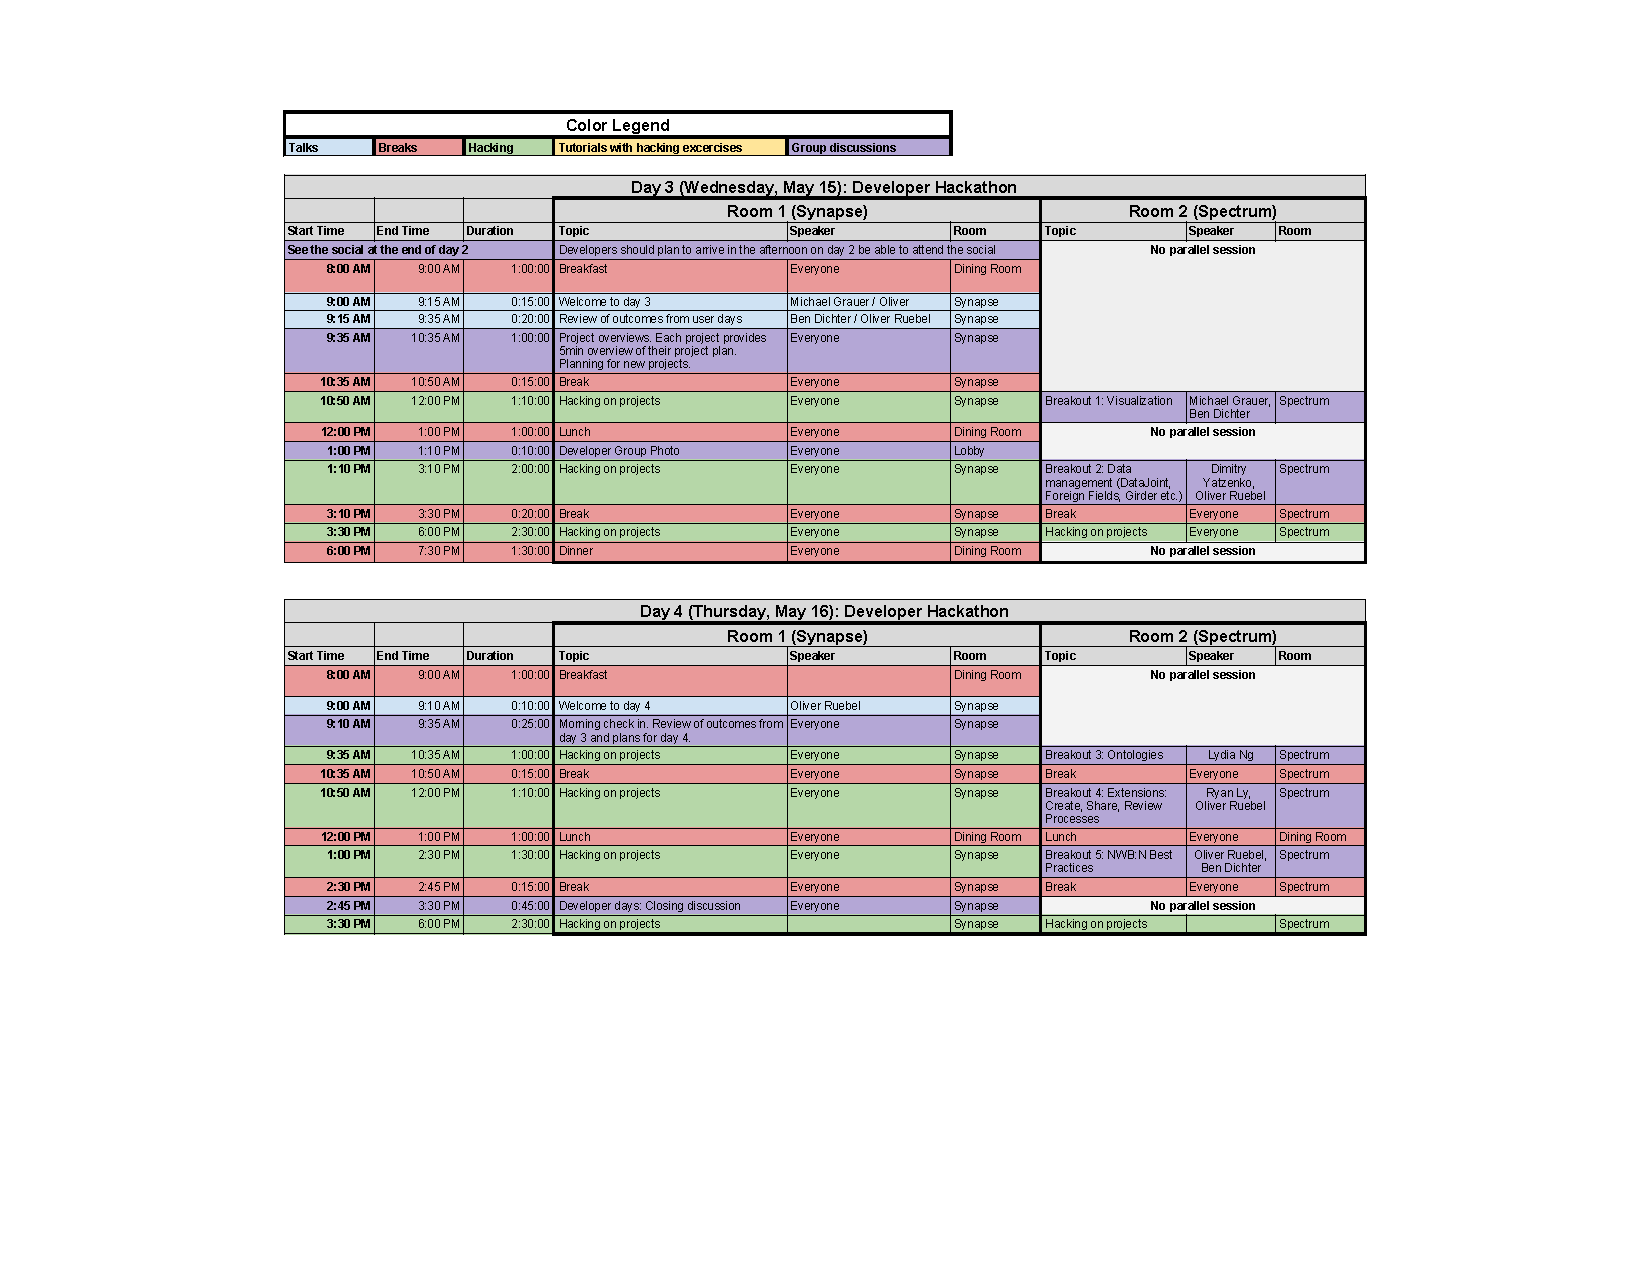
\includegraphics[width=\textwidth]{figures/agenda_developer_days.pdf}
\end{figure*}

\subsection{Time Breakdown}
\begin{figure*}[h!]
\centering
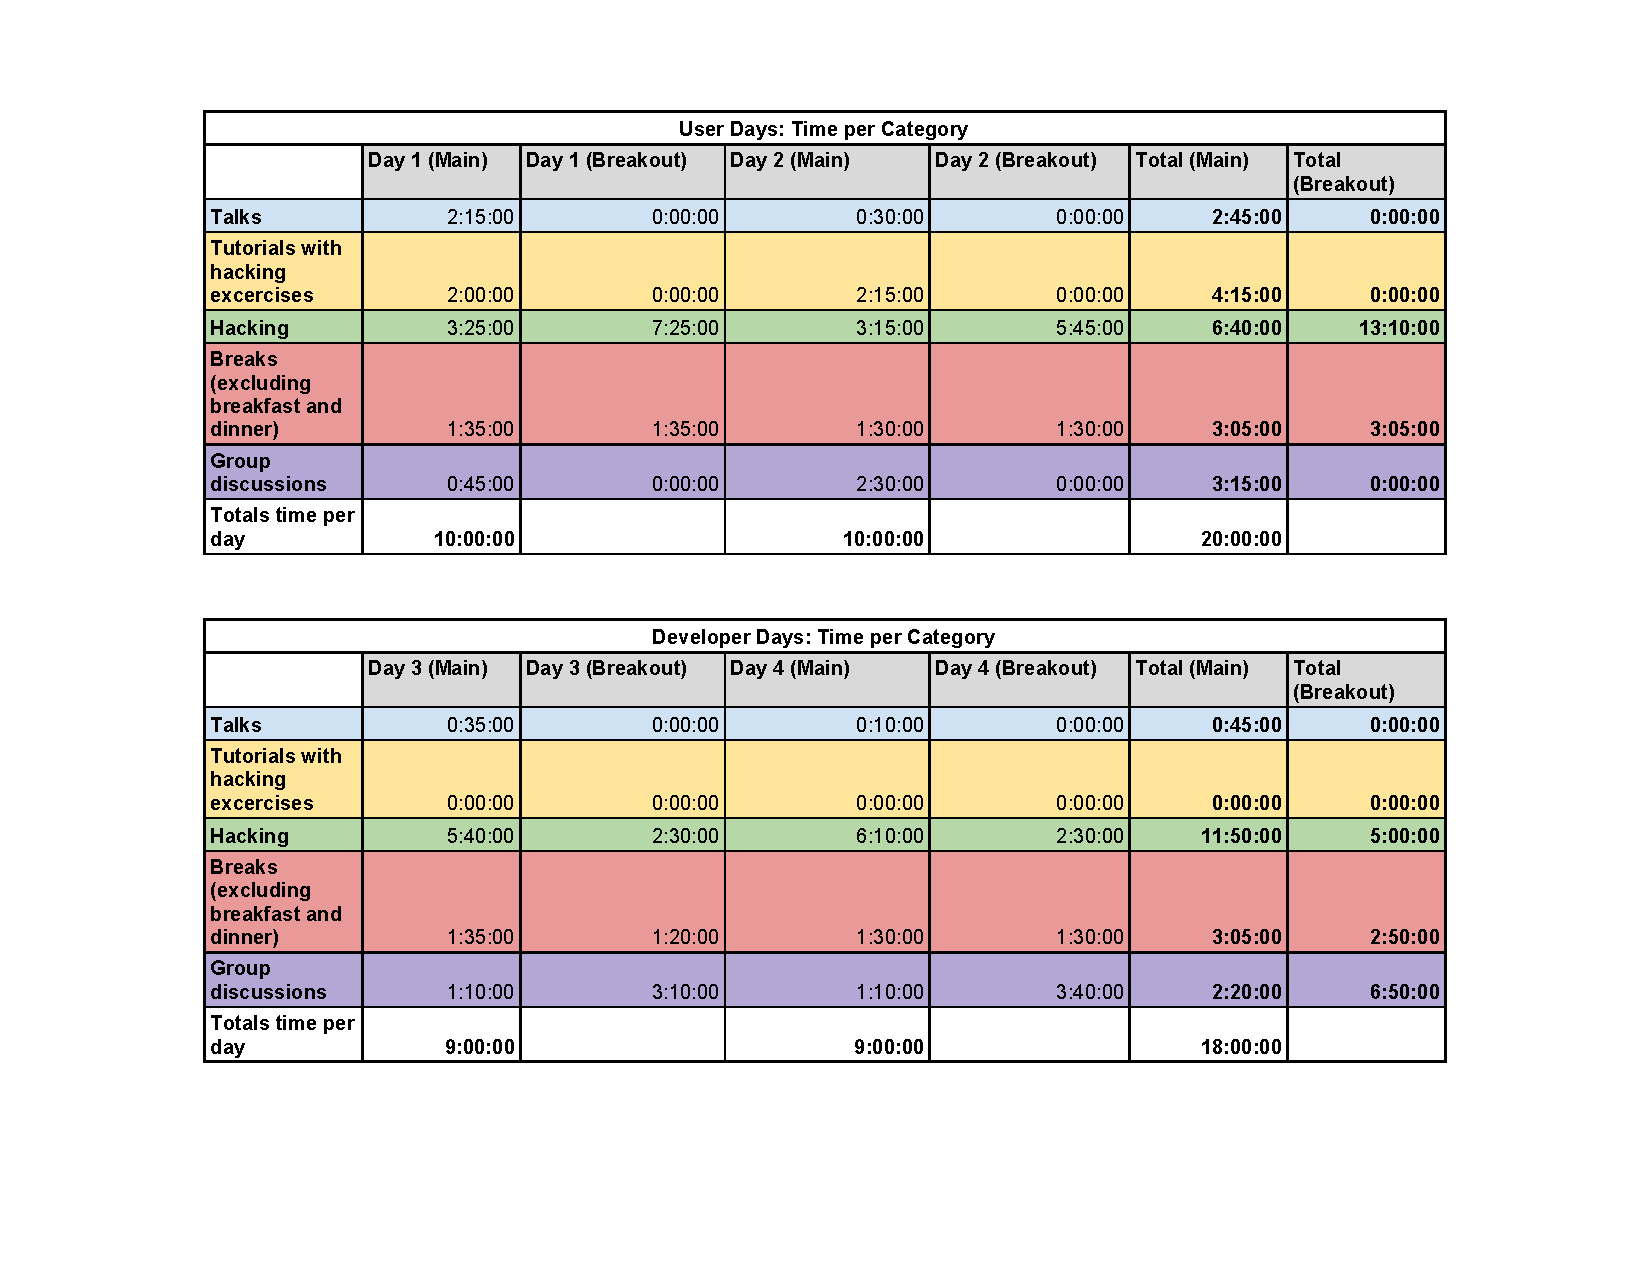
\includegraphics[width=11.5cm]{figures/agenda_time_breakdown.pdf}
\end{figure*}


\clearpage
\section{Hackathon Projects}
\label{sec:userprojects}

Prior to the event, each participant was asked by the organizers to formulate a specific project that 
she/he will work on. The participants created project pages on the \href{https://neurodatawithoutborders.github.io/nwb_hackathons/HCK06_2019_Janelia/#projects}{hackathon GitHub repository}. Participants then updated their pages during (and after) the event to document progress. In the following we provide a brief overview of the various projects. The project headings include links to the specific project pages
for further details. 

\subsection{Data Import/Convert}

\begin{enumerate}
    \item \href{https://neurodatawithoutborders.github.io/nwb_hackathons/HCK06_2019_Janelia/projects/BenderOptimization/}{Integrate neuron model optimization and simulation data with NWB:N} The goal of the project is to use NWB:N to store simulated neuron model data, as well as stimuli and parameter sets, instead of the current method of storing data in csv files. The project has made significant progress in identifying native NWB:N data structures to use, determining how best to organize data in NWB:N, learning how to use extensions for the simulation output, and integrating NWB:N with the stimulus generation code.
        \vspace{-0.2cm}
        \begin{itemize}[noitemsep]
            \item \textbf{Key Investigators:} Matthew T. Sit and Roy Ben-Shalom 
            \item \textbf{Key Institutions:} University of California Berkeley (UCB), University of Califorina San Francisco (UCSF), and Lawrence Berkeley National Laboratory (LBNL)
        \end{itemize}
        
    \item \href{https://neurodatawithoutborders.github.io/nwb_hackathons/HCK06_2019_Janelia/projects/x_to_nwb/}{Convert data in Abf and Dat formats to NWB:N} The \href{https://github.com/AllenInstitute/ipfx/tree/master/ipfx/x_to_nwb}{x\_to\_nwb} package has been developed to convert two of the most common formats for \textit{in vitro} physiology data -- $.abf$ (pClamp, Molecular Devices) and $.dat$ (PatchMaster, HEKA) -- into the NWB:N format. These tools are new and this project will be focused on investigating their compatibility. The objectives of this project include to 1) determine if there are any lingering issues to be addressed in the latest version of the abf and dat file to nwb converter and to 2) brainstorm strategies for increasing visibility of abf\_and\_dat\_to\_nwb functionality. The project has made significant progress in that: 1) the latest version of the converter works well with several recent example abf and dat files and 2) a list of ways to increase outreach has been started, which includes pulling the converter out of the ipfx package in the Allen SDK and giving it its own repo as well as making sure that the code is clear on the expectations for maintenance.
        \vspace{-0.2cm}
        \begin{itemize}[noitemsep]
            \item \textbf{Key Investigators:} Jim Berg and Thomas Braun
            \item \textbf{Key Institutions:} Allen Institute for Brain Science (AIBS) and byte physics
        \end{itemize}

    \item \href{https://neurodatawithoutborders.github.io/nwb_hackathons/HCK06_2019_Janelia/projects/changlab_to_nwb/}{Integrate ChangLab ECoG, behavioral, and imaging data with NWB:N} The Chang Lab records from a TDT acquisition system and has an in-house preprocessing pipeline for converting the raw TDT files into raw and preprocessed HTK files. The goal is to update this pipeline to be completely in Python and to utilize the NWB:N format. The objectives of this project include to: 1) Gain experience integrating the most common types of lab data (TDT/HTK, behavioral logs, imaging) into .nwb files and 2) be able to help lab members convert their data/be familiar with existing efforts to convert lab data to NWB:N format. Progress for this project include: 1) developed Python script for conversion of TDT to NWB:N files (including cortical surface using an extension), 2) stored frequency decomposition as DecompositionSeries, 3) used visualization tools with NWB:N files, 4) verified files. 
        \vspace{-0.2cm}
        \begin{itemize}[noitemsep]
            \item \textbf{Key Investigators:} Jessie R. Liu 
            \item \textbf{Key Institutions:} Chang Lab, UCSF
        \end{itemize}
        
    \item \href{https://neurodatawithoutborders.github.io/nwb_hackathons/HCK06_2019_Janelia/projects/NMRC/}{Integrate data from the Neuromodulation Research Center (UMN)} The goal of this project is to integrate all types of data from the Neuromodulation Research Center with NWB:N, including 1) raw data from TDT recording system, 2) raw behavioral and motion analysis system data (e.g., touch pad and eye movement data), 3) pre-processed data and 4) general experiment metadata. Accomplishments as part of the hackathon include: 1) converted raw data from TDT, 2) converted data from motion analysis system, and 3) learned details about the structure and usage of NWB:N. 
        \vspace{-0.2cm}
        \begin{itemize}[noitemsep]
            \item \textbf{Key Investigators:} Lingling Yang 
            \item \textbf{Key Institutions:} University of Minnesota
        \end{itemize}
        
    \item \href{https://neurodatawithoutborders.github.io/nwb_hackathons/HCK06_2019_Janelia/projects/kanoldLabNWB/}{Integrate Thorlabs 2-photon calcium imaging data with NWB} The Kanold lab at UMD uses 2-photon calcium imaging to study the auditory cortex. The goal is to convert 2-photon calcium imaging data, both raw and processed, into the NWB:N format in order to have a generalized output from the Thorlabs microscope. Accomplishments as part of the hackathon include: 1) converted raw and registered imaging data as well as experimental metadata to NWB, 2) learned about structure and usage of NWB:N for imaging and behavioral data.
        \vspace{-0.2cm}
        \begin{itemize}[noitemsep]
            \item \textbf{Key Investigators:} Zac Bowen and Kelson Shilling-Scrivo
            \item \textbf{Key Institutions:} University of Maryland
        \end{itemize}
        
    \item \href{https://neurodatawithoutborders.github.io/nwb_hackathons/HCK06_2019_Janelia/projects/tandonlab2NWB/}{Convert Tandon lab ECoG data to NWB} 
        \vspace{-0.2cm}
        \begin{itemize}[noitemsep]
            \item \textbf{Key Investigators:} Oscar Woolnough
            \item \textbf{Key Institutions:} University of Texas
        \end{itemize}
        
    \item \href{https://neurodatawithoutborders.github.io/nwb_hackathons/HCK06_2019_Janelia/projects/RutishauserLab2NWB/}{Convert Rutishauser lab data to NWB} The goal of the project is to convert native Rutishauser lab data -- electrophysiology and behavior -- into the NWB:N format and modify the existing analysis pipeline to use NWB.
        \vspace{-0.2cm}
        \begin{itemize}[noitemsep]
            \item \textbf{Key Investigators:} Nand Chandravadia
            \item \textbf{Key Institutions:} Cedars-Sinai
        \end{itemize}
        
    \item \href{https://neurodatawithoutborders.github.io/nwb_hackathons/HCK06_2019_Janelia/projects/Zuckerman2NWB/}{Create demonstration code to convert data from Zuckerman Institute to NWB} The goal of the project is to demonstrate to the Zuckerman Institute’s faculty and their labs, associated with one of the two U19 projects (Costa and Miller), that data routinely used in data processing pipelines in the labs can be readily converted into and stored as NWB:N files. The objectives include identifying the mapping between existing metadata and NWB:N fields, creating a first-pass converter each of five datasets, and testing that NWB:N data can be read back and interchanged between Python and Matlab environments.
        \vspace{-0.2cm}
        \begin{itemize}[noitemsep]
            \item \textbf{Key Investigators:} Jochen Weber
            \item \textbf{Key Institutions:} Columbia Zuckerman Institute
        \end{itemize}
        
    \item \href{https://neurodatawithoutborders.github.io/nwb_hackathons/HCK06_2019_Janelia/projects/singleCell_PhysiologyImaging/}{Integrate simultaneously recorded single-cell physiology and imaging data with NWB} The goals of the project are to integrate single-cell physiology and imaging data in NWB:N and create an extension for kymograph data.
        \vspace{-0.2cm}
        \begin{itemize}[noitemsep]
            \item \textbf{Key Investigators:} Andrew Landau
            \item \textbf{Key Institutions:} Harvard Medical School
        \end{itemize}
        
    \item \href{https://neurodatawithoutborders.github.io/nwb_hackathons/HCK06_2019_Janelia/projects/BuzsakiLab2NWB/}{Convert Buzsaki lab data to NWB} The goal of the project is to generate scripts that load data stored in an internal lab data format (“buzcode”) to NWB.
        \vspace{-0.2cm}
        \begin{itemize}[noitemsep]
            \item \textbf{Key Investigators:} Roman Huszar and Peter Petersen
            \item \textbf{Key Institutions:} New York University
        \end{itemize}
        
    \item \href{https://neurodatawithoutborders.github.io/nwb_hackathons/HCK06_2019_Janelia/projects/Mesoscale_Activity_Project_to_NWB/}{Convert Mesoscale Activity Project data to NWB} The goal of the project is to design export tools for the \href{https://github.com/vathes/map-ephys}{Mesoscale Activity Project} into NWB. This involves first mapping DataJoint schema into the NWB:N format and then developing automatic export routines. 
        \vspace{-0.2cm}
        \begin{itemize}[noitemsep]
            \item \textbf{Key Investigators:} Dimitriy Yatsenko and Thinh Nguyen
            \item \textbf{Key Institutions:} Vathes LLC
        \end{itemize}
        
    \item \href{https://neurodatawithoutborders.github.io/nwb_hackathons/HCK06_2019_Janelia/projects/bmtk_nwb/}{Convert Brain Modeling Toolkit output to NWB} The goal of the project is to use NWB:N as an output format for the Brain Modeling Toolkit to record cell variables, utilizing the NWB:N simulation\_output extension produced at a previous hackathon.
        \vspace{-0.2cm}
        \begin{itemize}[noitemsep]
            \item \textbf{Key Investigators:} Vyassa Baratham
            \item \textbf{Key Institutions:} LBNL
        \end{itemize}
        
    \item \href{https://neurodatawithoutborders.github.io/nwb_hackathons/HCK06_2019_Janelia/projects/AcquisitionSystemImporters/}{Import data from acquisition systems} The objectives of this project include adding support and writing conversion scripts for the following acquisition systems: TDT, Plexon, Intan, Ripple, and Blackrock. 
        \vspace{-0.2cm}
        \begin{itemize}[noitemsep]
            \item \textbf{Key Investigators:} Konstantinos Nasiotis
            \item \textbf{Key Institutions:} McGill University
        \end{itemize}
        
    % Remember the project counter so we can continue to enumerate our project list
    \newcounter{projectEnumCounter}
    \setcounter{projectEnumCounter}{\theenumi}
\end{enumerate}

\subsection{Data Storage and Management}

\begin{enumerate}
    \setcounter{enumi}{\theprojectEnumCounter}  % Restore our project enumeration counter
    \item \href{https://neurodatawithoutborders.github.io/nwb_hackathons/HCK06_2019_Janelia/projects/ZARR/}{Integrate ZARR with HDMF/PyNWB}  The goal of this project is to integrate ZARR as an I/O backend with HDMF.
        \vspace{-0.2cm}
        \begin{itemize}[noitemsep]
            \item \textbf{Key Investigators:} Donghe Kang and Oliver R\"ubel
            \item \textbf{Key Institutions:} Ohio State University and LBNL
        \end{itemize}
        
    \item \href{https://neurodatawithoutborders.github.io/nwb_hackathons/HCK06_2019_Janelia/projects/Exdir/}{Implement Exdir as an alternative backend to HDF5}  Exdir is a hierarchical data structure similar to HDF5 which operates on the filesystem instead of a HDF5 file.  Having Exdir as a backend in NWB:N would enable users to operate directly on the filesystem, which would facilitate human readability of metadata and may work better with version control systems such as git and sharing of partial data sets. The goals of this project are to implement object and region references in Exdir and to then implement a working version of Exdir in HDMF. 
        \vspace{-0.2cm}
        \begin{itemize}[noitemsep]
            \item \textbf{Key Investigators:} Mikkel Elle Lepperød
            \item \textbf{Key Institutions:} CINPLA, University of Oslo, Norway
        \end{itemize}
    
    \item \href{https://neurodatawithoutborders.github.io/nwb_hackathons/HCK06_2019_Janelia/projects/NIX/}{Evaluate possible integration between NIX and NWB:N} The goal of the project is to explore possibilities for integration between the NIX and NWB:N standards and software ecosystems, including conversion of select data types between NIX and NWB:N and identification of possible avenues for future collaboration between NIX and NWB. 
        \vspace{-0.2cm}
        \begin{itemize}[noitemsep]
            \item \textbf{Key Investigators:} Christian Kellner and Oliver R\"ubel
            \item \textbf{Key Institutions:} G-Node, Red Hat, and LBNL
        \end{itemize}
    
    % Remember the project counter so we can continue to enumerate our project list
    \setcounter{projectEnumCounter}{\theenumi}
\end{enumerate}

\subsection{Data Analysis and Visualization}

\begin{enumerate}
    \setcounter{enumi}{\theprojectEnumCounter}  % Restore our project enumeration counter
    \item \href{https://neurodatawithoutborders.github.io/nwb_hackathons/HCK06_2019_Janelia/projects/RAVE/}{Integrate NWB:N with RAVE}  The goal of this project is to create “R” code that will allow our ECOG package, RAVE, to read in (as a start) voltage traces from NWB:N files. Progress for this project include development of a working converter script for reading NWB:N files into RAVE and a \href{https://youtu.be/h_W9FyHKokA}{working visualization demo} with ECoG data stored in NWB.
        \vspace{-0.2cm}
        \begin{itemize}[noitemsep]
            \item \textbf{Key Investigators:} Zhengjia Wang
            \item \textbf{Key Institutions:} Baylor College of Medicine
        \end{itemize}

    \item \href{https://neurodatawithoutborders.github.io/nwb_hackathons/HCK06_2019_Janelia/projects/JupyterWidgets/}{NWB:N Jupyter widgets} The \href{https://github.com/NeurodataWithoutBorders/nwb-jupyter-widgets/}{nwbwidgets project} allows for interactive exploration of an NWB:N file with built-in plotting of recognized data types within Jupyter. The goal of the project is to detect when an ECoG cortical surfaces is stored in an NWB:N file and create a 3D, interactive visualization of the surface. Considerable progress was made in \href{https://camo.githubusercontent.com/6409f891a8591f2799b4d8cbfb4899cf2014bc52/68747470733a2f2f692e696d6775722e636f6d2f423939676838312e676966}{visualizing behavioral data} from the Allen Institute, and some progress was made in visualizing a cortical surface. 
        \vspace{-0.2cm}
        \begin{itemize}[noitemsep]
            \item \textbf{Key Investigators:} Matt McCormick and Ben Dichter
            \item \textbf{Key Institutions:} Kitware and LBNL
        \end{itemize}
        
    \item \href{https://neurodatawithoutborders.github.io/nwb_hackathons/HCK06_2019_Janelia/projects/OSB_NWB_Explorer/}{Visualizing contents of NWB:N files with NWB Explorer and Open Source Brain} \href{http://opensourcebrain.org/}{Open Source Brain} is an open source, web-based resource for visualizing, simulating and disseminating standardized models of neurons and circuits from many brain regions. The primary goal at this hackathon is to gather existing NWB:N datasets to check and improve compatibility with the basic parser of NWB Explorer, determine scientifically useful workflows and the components necessary to support them, and develop a basic widget for exposing in a readable fashion the structure of an NWB:N file. The approach includes collecting example datasets and conversion scripts for the \href{https://github.com/OpenSourceBrain/NWBShowcase}{NWB Showcase}, and assessing attendee demand for functionality in NWB Explorer. 
        \vspace{-0.2cm}
        \begin{itemize}[noitemsep]
            \item \textbf{Key Investigators:} Matt Earnshaw, Padraig Gleeson, and Matteo Cantarelli Gleeson
            \item \textbf{Key Institutions:} University College London and MetaCell
        \end{itemize}
        
    % Remember the project counter so we can continue to enumerate our project list
    \setcounter{projectEnumCounter}{\theenumi}
\end{enumerate}


\subsection{Core Development and Documentation}

\begin{enumerate}
    \setcounter{enumi}{\theprojectEnumCounter}  % Restore our project enumeration counter
            
    \item \href{https://neurodatawithoutborders.github.io/nwb_hackathons/HCK06_2019_Janelia/projects/lazy_cross_file_links/}{Implement lazy cross-file links} The Allen plans to release large data sets in the NWB:N format. The goal of the project is to enable downloading of components of an NWB:N file, e.g. only the LFP data from multiple neuropixels probes. 
        \vspace{-0.2cm}
        \begin{itemize}[noitemsep]
            \item \textbf{Key Investigators:} Nile Graddis
            \item \textbf{Key Institutions:} AIBS
        \end{itemize}
    
    \item \href{https://neurodatawithoutborders.github.io/nwb_hackathons/HCK06_2019_Janelia/projects/UseCaseGathering/}{Use case gathering} The goal of the project is to collect experimental and analysis use cases from participants of the User Days to inform community needs in the development of controlled vocabularies and ontologies. Progress for this project include interviews of five groups of users and creation of a \href{https://github.com/NeurodataWithoutBorders/ontology-project/tree/master/use-cases}{GitHub repo} to store the interview summaries.
        \vspace{-0.2cm}
        \begin{itemize}[noitemsep]
            \item \textbf{Key Investigators:} Lydia Ng, Michael Grauer
            \item \textbf{Key Institutions:} AIBS, Kitware
        \end{itemize}
        
    \item \href{https://neurodatawithoutborders.github.io/nwb_hackathons/HCK06_2019_Janelia/projects/ExtensionSharing/}{Develop infrastructure for extension sharing}  The goal of the project is to evaluate plans for infrastructure for web-based sharing, deployment, and evaluation of extensions, and also develop the infrastructure for the online archive of NWB:N extensions. Progress for this project include receiving feedback from developers on the user flowchart for developing, sharing, and deploying extensions, adding continuous integration using Azure Pipelines to the \href{https://github.com/nwb-extensions/ndx-template}{ndx-template} repo and related repos, consolidating documentation, reviewing conda-forge infrastructure, and planning continuous integration and automation for the \href{https://github.com/nwb-extensions/staged-extensions}{staged-extensions} repo.
        \vspace{-0.2cm}
        \begin{itemize}[noitemsep]
            \item \textbf{Key Investigators:} Ryan Ly, Jean-Christophe Fillion-Robin, Oliver R\"ubel, Andrew Tritt, and Ben Dichter
            \item \textbf{Key Institutions:} LBNL, Kitware
        \end{itemize}
        
    \item \href{https://neurodatawithoutborders.github.io/nwb_hackathons/HCK06_2019_Janelia/projects/DataJoint_NWB_Interoperability/}{DataJoint-NWB-Interoperability}  DataJoint is a data processing pipeline management system that has been successful in various large-scale neuroscience collaborations. The objectives of this project include discussing how to integrate DataJoint with NWB:N to make them interoperable; that is, how to allow data stored in NWB:N to be used with DataJoint, and how to  export data from DataJoint to NWB. Progress includes discussion of four possible routes for DataJoint-NWB integration: 1. through DataJoint canonical pipelines, 2. by using NWB:N datatypes in DataJoint and implementing an archival adapter, 3. by inferring DataJoint schemas from NWB:N types and using DataJoint as a back-end, and 4. by building DataJoint schemas using a DataJoint schema template inferred from the NWB:N YAML schema files plus human intervention. Of these, options 4 and 1 were the most promising and will be explored further. 
        \vspace{-0.2cm}
        \begin{itemize}[noitemsep]
            \item \textbf{Key Investigators:} Dimitri Yatsenko, Thinh Nguyen, Andrew Tritt, and Oliver R\"ubel
            \item \textbf{Key Institutions:} Vathes LLC, LBNL
        \end{itemize}
    
    \item \href{https://neurodatawithoutborders.github.io/nwb_hackathons/HCK06_2019_Janelia/projects/NWBIndex/}{NWBIndex}  The NWBIndex project is intended to help with the problem of sharing NWB:N files, to allow for discoverability, browsing, search, and accessibility. It is a long-range project intended to build tools to index existing NWB:N files and provide guidance to groups wanting to share their data. The primary goal for this hackathon, similar to the OSB NWB Explorer Project, is to gather examples of NWB:N datasets and forge collaborations with groups producing and consuming NWB:N data. The approach is to meet with participants to ask about NWB:N data for sharing and data sharing needs; collect public datasets along with metadata, and ideas about useful visual summaries; discuss with participants current approaches and pain points to sharing data, and find commonalities; and understand participants’ data release plans, build collaborations to improve usability and discoverability of that data.
        \vspace{-0.2cm}
        \begin{itemize}[noitemsep]
            \item \textbf{Key Investigators:} Mike Grauer
            \item \textbf{Key Institutions:} Kitware
        \end{itemize}
    
    \item \href{https://neurodatawithoutborders.github.io/nwb_hackathons/HCK06_2019_Janelia/projects/NWB_Query/}{Query and complex indexing for NWB:N data}  The objectives of this project is to develop an implementation plan for query/complex slicing in NWB. It was discussed how to enhance or rewrite the Query class of HDMF to take and perform slices on a target, e.g. TimeSeries, add defined-over/domain/support/observation-intervals to TimeSeries class, add an abstract Mask class to HDMF, and add a class to represent list of non-overlapping intervals. The next step is to move these into GitHub as issues, and start writing code.
        \vspace{-0.2cm}
        \begin{itemize}[noitemsep]
            \item \textbf{Key Investigators:} Andrew Tritt, Tom Davidson, and Nile Graddis
            \item \textbf{Key Institutions:} LBNL, UCSF, AIBS
        \end{itemize}
    
    \item \href{https://neurodatawithoutborders.github.io/nwb_hackathons/HCK06_2019_Janelia/projects/greatly-enhance-documentation/}{Greatly enhance documentation}  The documentation currently does not link to internal types and some external types accessible via intersphinx. Progress for the project include \href{https://github.com/NeurodataWithoutBorders/pynwb/pull/938}{major} \href{https://github.com/hdmf-dev/hdmf/pull/61}{fixes} to this issue, which have since been merged into the main codebase.
        \vspace{-0.2cm}
        \begin{itemize}[noitemsep]
            \item \textbf{Key Investigators:} Thomas Braun
            \item \textbf{Key Institutions:} byte physics
        \end{itemize}
    
    \item \href{https://neurodatawithoutborders.github.io/nwb_hackathons/HCK06_2019_Janelia/projects/validation-enhancements/}{Enhance the validation tool}  The validation tool currently does not support checking against a stored specification. In addition, it does not warn about unknown entries in the NWB:N file. Progress for the project include discussing how to best handle various issues with the validator.
        \vspace{-0.2cm}
        \begin{itemize}[noitemsep]
            \item \textbf{Key Investigators:} Thomas Braun
            \item \textbf{Key Institutions:} byte physics
        \end{itemize}
           
    \item \href{https://neurodatawithoutborders.github.io/nwb_hackathons/HCK06_2019_Janelia/projects/Interactive_PyNWB_Course/}{Interactive PyNWB Course} Users described a large learning curve for understanding the NWB:N format and using the APIs. The goal of the project is to create a more beginner-friendly, interactive tutorial/mini-course on NWB, starting with PyNWB. Open-source software was used to develop the interactive course, and an existing tutorial was adapted to become Chapter 1. A live demo of the course is linked \href{https://pynwb-course.netlify.com/}{here}.
        \vspace{-0.2cm}
        \begin{itemize}[noitemsep]
            \item \textbf{Key Investigators:} Ryan Ly and Ben Dichter
            \item \textbf{Key Institutions:} LBNL
        \end{itemize}
        
    \item \href{https://neurodatawithoutborders.github.io/best_practices}{Develop list of best practices} To enable NWB:N to accommodate the needs of the diverse neuroscience community, NWB:N provides a great degree of flexibility. While this flexibility is essential to enable coverage of a broad range of use-cases, it can also lead to ambiguity. Developers and experienced users came together during a Developer Days breakout session to create a \href{https://neurodatawithoutborders.github.io/best_practices}{list of best practices}, which outlines some of the pitfalls to avoid and common usage patterns to emulate. 
        \vspace{-0.2cm}
        \begin{itemize}[noitemsep]
            \item \textbf{Key Investigators:} Oliver R\"ubel, Andrew Tritt, Ben Dichter, Ryan Ly, Thomas Braun, Tom Davidson, Nicholas Cain, Lydia Ng
            \item \textbf{Key Institutions:} LBNL, byte physics, UCSF, Allen Institute
        \end{itemize}
        
    % Remember the project counter so we can continue to enumerate our project list
    \setcounter{projectEnumCounter}{\theenumi}
\end{enumerate}

\clearpage
\section{Code Activity (May 2019)}

The hackathon has helped to create a lot of energy around the NWB:N main repositories. Here we report GitHub 
code statistics for the main NWB:N repositories\footnote{\textbf{Note:} The statistics reported here focus on the main NWB:N repositories only. A majority of hackathon projects involved external data analysis, visualization, storage, and management tools and custom user codes (e.g,. for data conversion) as well as new NWB:N code repositories, e.g., for the 1) \href{https://github.com/NeurodataWithoutBorders/pynwb-course}{PyNWB interactive course}, 2) \href{https://github.com/NeurodataWithoutBorders/ontology-project}{ontology project}, 3) \href{https://github.com/NeurodataWithoutBorders/nwb-jupyter-widgets}{NWB:N jupyter widgets}, and the 4) \href{https://github.com/nwb-extensions}{NWB:N extension catalog},  which are not reflected here.} for the period of 04/30/2019 -- 05/30/2019 (10:30am), with the User Days (May 13-14) and Developer Days (May 15-16) being roughly in the middle of that period.

\subsection{NWB:N Software Repositories}

The charts below summarize activity on the main NWB:N code repositories for 1) \href{https://github.com/NeurodataWithoutBorders/pynwb}{PyNWB}, 2) \href{https://github.com/NeurodataWithoutBorders/pynwb}{HDMF}, 3) \href{https://github.com/NeurodataWithoutBorders/matnwb}{MatNWB}, 4) \href{https://github.com/NeurodataWithoutBorders/nwb-schema}{NWB:N Schema}, and the 5) \href{https://github.com/NeurodataWithoutBorders/nwb-docutils}{Documentation Utilities}. Across these NWB:N codes we have seen significant progress on features and identification and resolution of issues, with \textbf{61} merged and \textbf{18} proposed pull requests and \textbf{35} closed and \textbf{46} new issues in the 30 day period reported here.

\begin{figure}[h!]
  \begin{minipage}[c]{0.67\textwidth}
    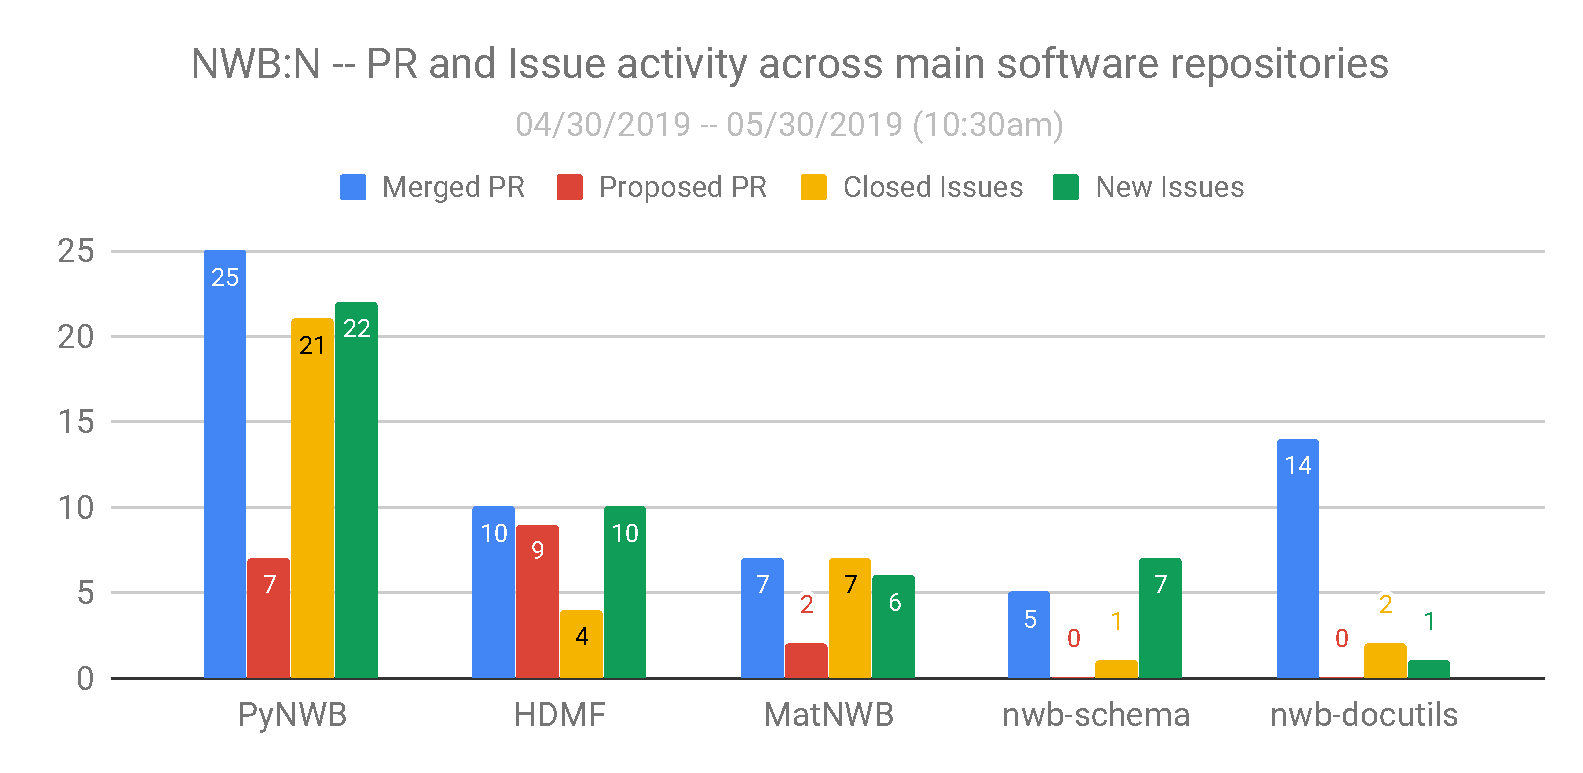
\includegraphics[width=\textwidth]{figures/nwbn_activity_software_pr_issues.pdf}
  \end{minipage}\hfill
  \begin{minipage}[c]{0.3\textwidth}
    \caption*{Pull request (PR) and issue activity across the main NWB:N software repositories in May 2019. In total there were \textbf{61} merged PR, \textbf{18} proposed PR, \textbf{35} closed issues, and \textbf{46} new issues.} 
  \end{minipage}
  \vspace{-0.3cm}
\end{figure}

\begin{figure}[h!]
  \begin{minipage}[c]{0.67\textwidth}
    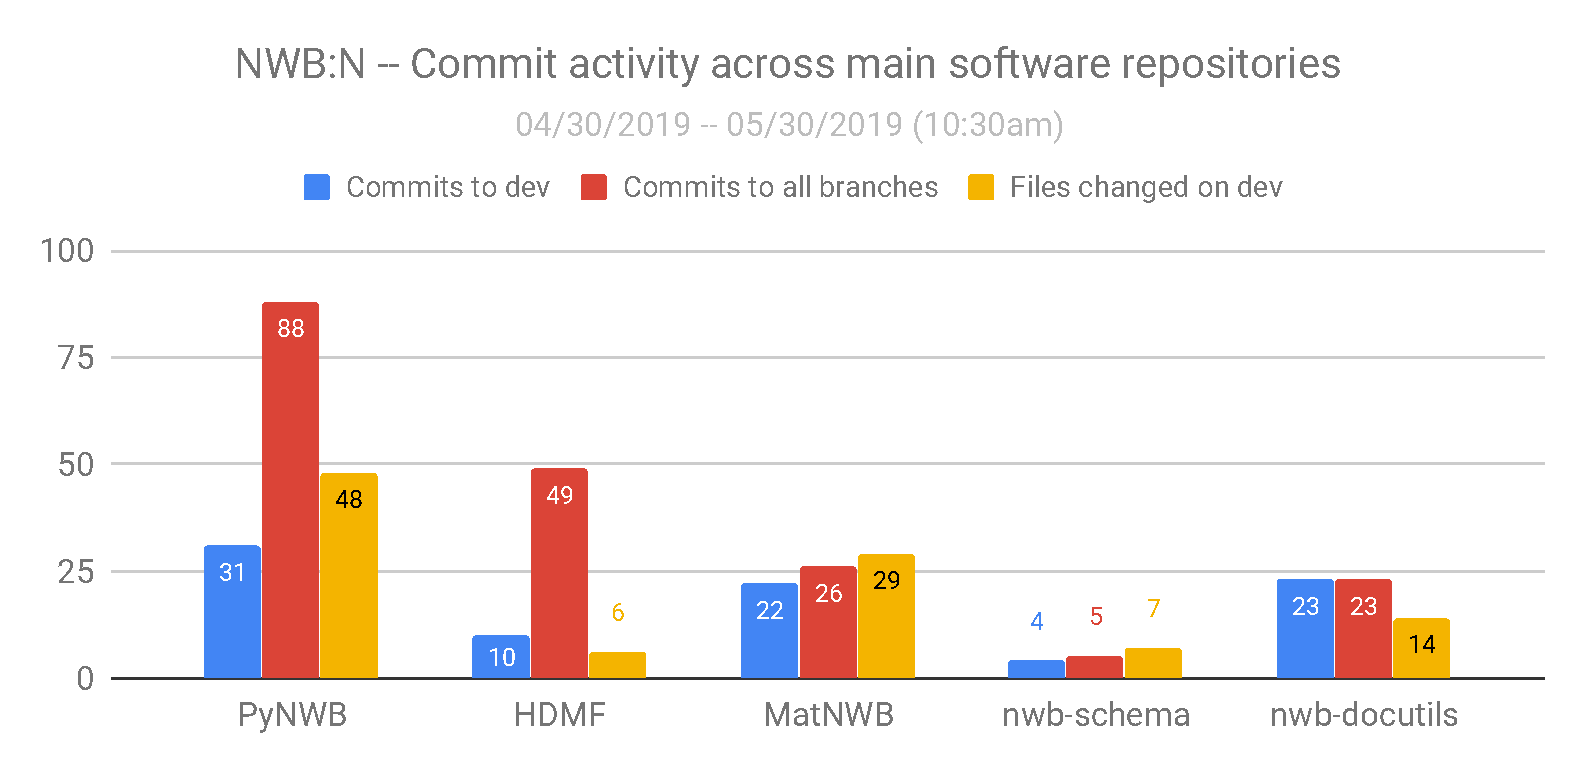
\includegraphics[width=\textwidth]{figures/nwbn_activity_software_commits_files.pdf}
  \end{minipage}\hfill
  \begin{minipage}[c]{0.3\textwidth}
    \caption*{Number of commits and files changed across the main NWB:N software repositories in May 2019. In total there were \textbf{191} commits and \textbf{104} files changed.} 
  \end{minipage}
\vspace{-0.3cm}
\end{figure}

\begin{figure}[h!]
  \begin{minipage}[c]{0.67\textwidth}
    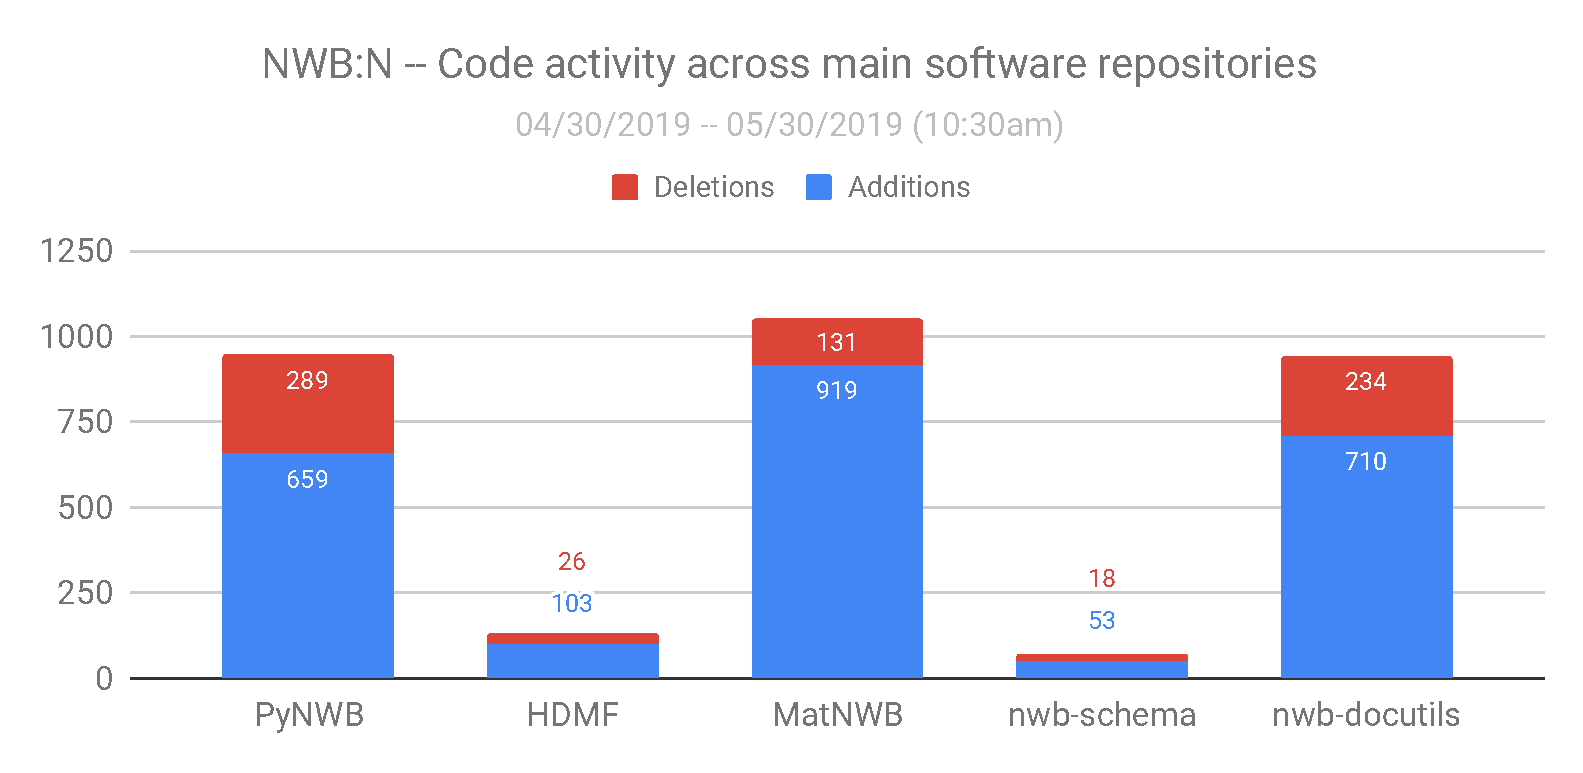
\includegraphics[width=\textwidth]{figures/nwbn_activity_software_code.pdf}
  \end{minipage}\hfill
  \begin{minipage}[c]{0.3\textwidth}
    \caption*{Code activity across the main NWB:N software repositories in May 2019. In total
there were \textbf{2,444} additions and \textbf{698} deletions.} 
  \end{minipage}
\vspace{-2cm}
\end{figure}



\clearpage
\subsection{NWB:N Website}

The charts below summarize activity on the main \href{https://neurodatawithoutborders.github.io/}{neurodatawithoutborders.github.io} as well as the \href{https://neurodatawithoutborders.github.io/hackathon_events}{hackathon} event page. As a result of the User Days and Developer Days we have seen significant improvements to the main website, in particular the addition of 1) \href{https://neurodatawithoutborders.github.io/best_practices}{Best Practices}, 2) \href{https://neurodatawithoutborders.github.io/exampledata}{Example NWB:N Data Files}, and 3) \href{https://neurodatawithoutborders.github.io/tools}{Analysis and Vis Tools} pages as well as 4) 30 different \href{https://neurodatawithoutborders.github.io/nwb_hackathons/HCK06_2019_Janelia/#projects}{hackathon project} pages. 

\begin{figure}[h!]
  \begin{minipage}[c]{0.67\textwidth}
    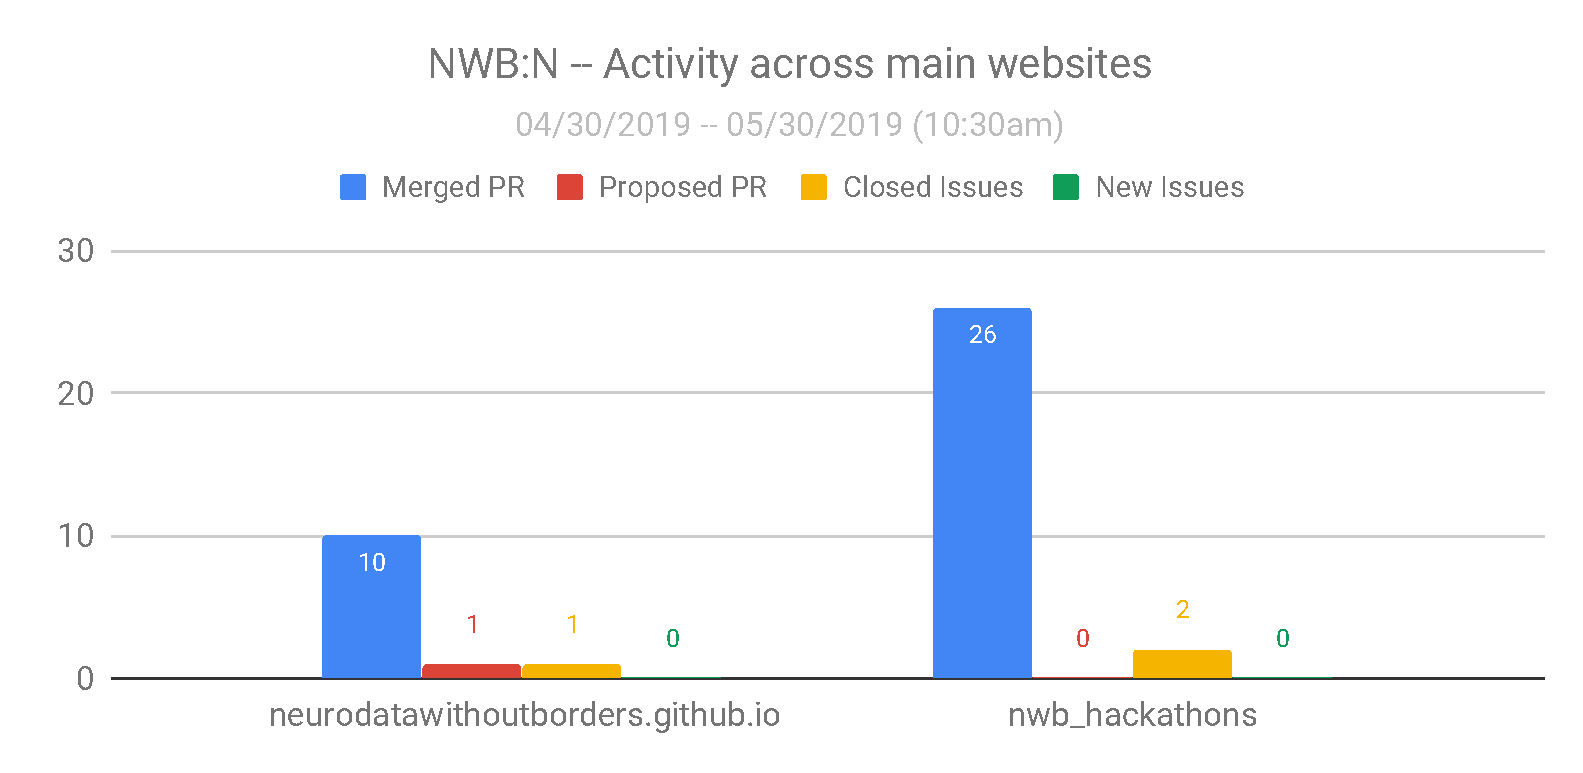
\includegraphics[width=\textwidth]{figures/nwbn_activity_websites_pr_issues.pdf}
  \end{minipage}\hfill
  \begin{minipage}[c]{0.3\textwidth}
    \caption*{Pull request (PR) and issue activity on \href{https://neurodatawithoutborders.github.io/}{neurodatawithoutborders.github.io} in May 2019. In total there were \textbf{36} merged PR, \textbf{1} proposed PR, \textbf{3} closed issues, and \textbf{0} new issues.} 
  \end{minipage}
\end{figure}

\begin{figure}[h!]
  \begin{minipage}[c]{0.67\textwidth}
    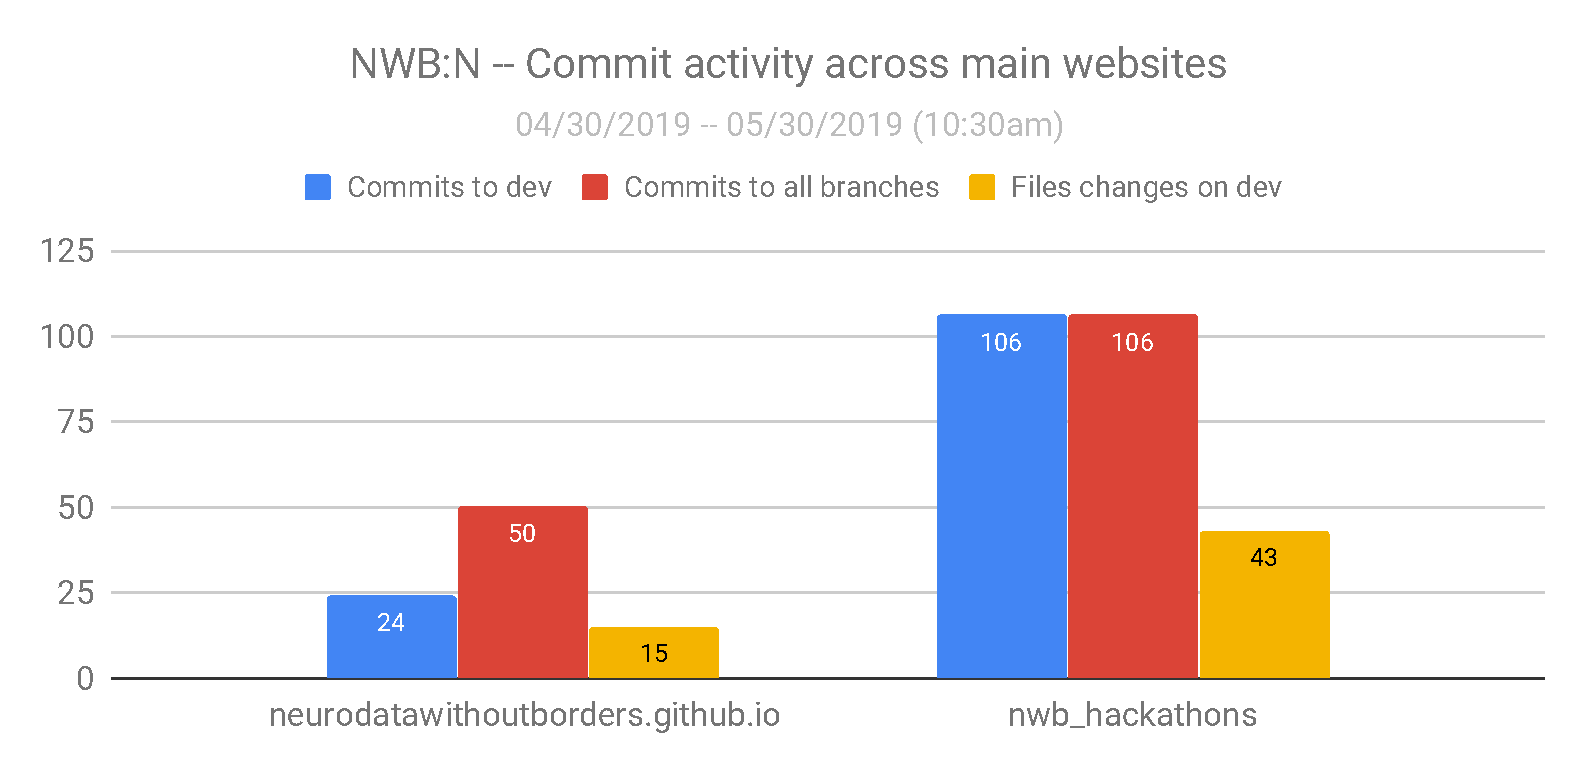
\includegraphics[width=\textwidth]{figures/nwbn_activity_websites_commits_files.pdf}
  \end{minipage}\hfill
  \begin{minipage}[c]{0.3\textwidth}
    \caption*{Number of commits and files changed on \href{https://neurodatawithoutborders.github.io/}{neurodatawithoutborders.github.io} in May 2019. In total there were \textbf{156} commits and \textbf{58} files changed.} 
  \end{minipage}
\end{figure}

\begin{figure}[h!]
  \begin{minipage}[c]{0.67\textwidth}
    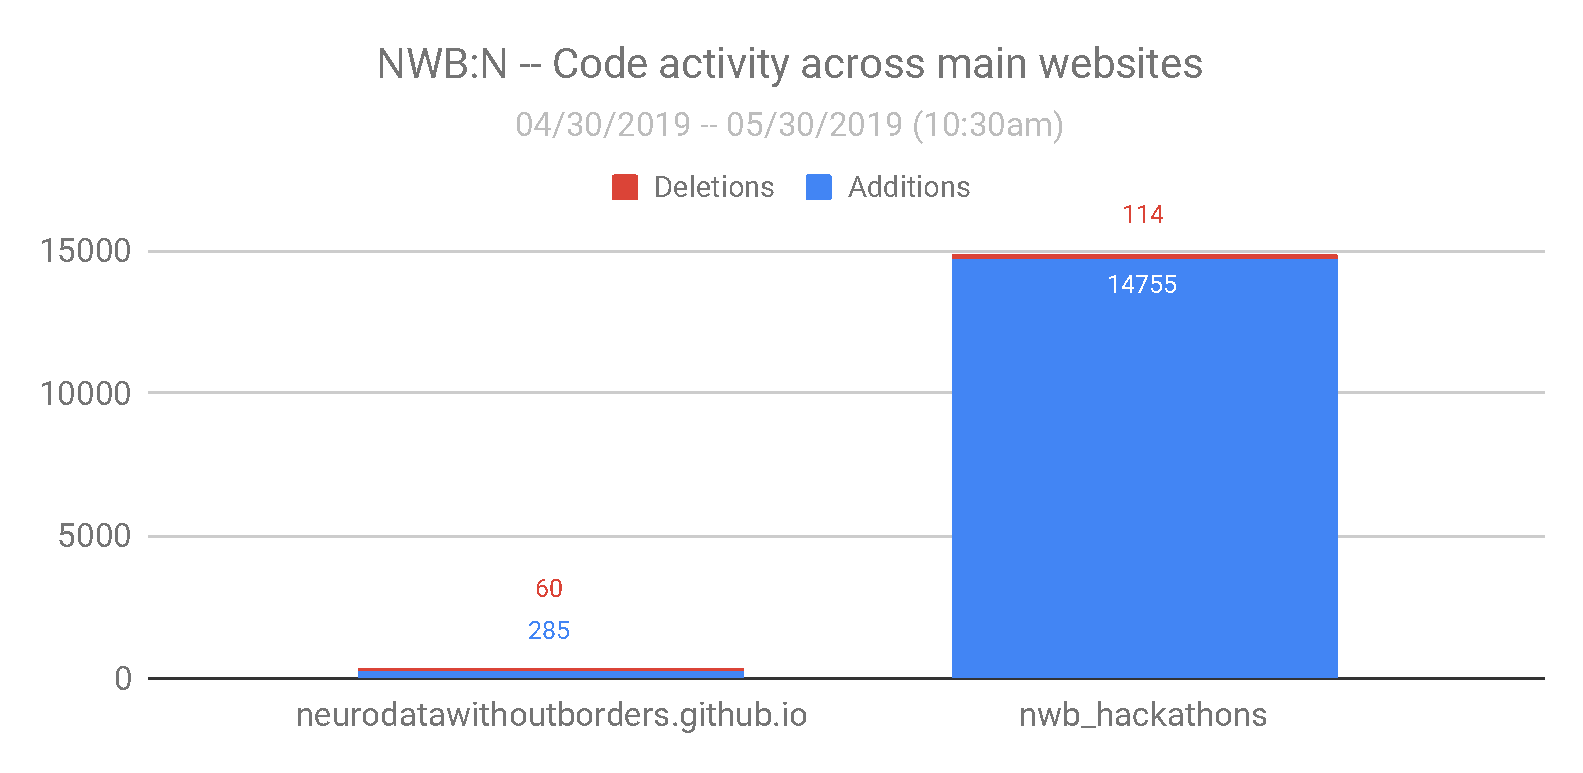
\includegraphics[width=\textwidth]{figures/nwbn_activity_websites_code.pdf}
  \end{minipage}\hfill
  \begin{minipage}[c]{0.3\textwidth}
    \caption*{Code activity on \href{https://neurodatawithoutborders.github.io/}{neurodatawithoutborders.github.io} in May 2019. In total
there were \textbf{15,040} additions and \textbf{174} deletions.} 
  \end{minipage}
\end{figure}


\clearpage
\section{Event Photos}

\begin{figure*}[h!]
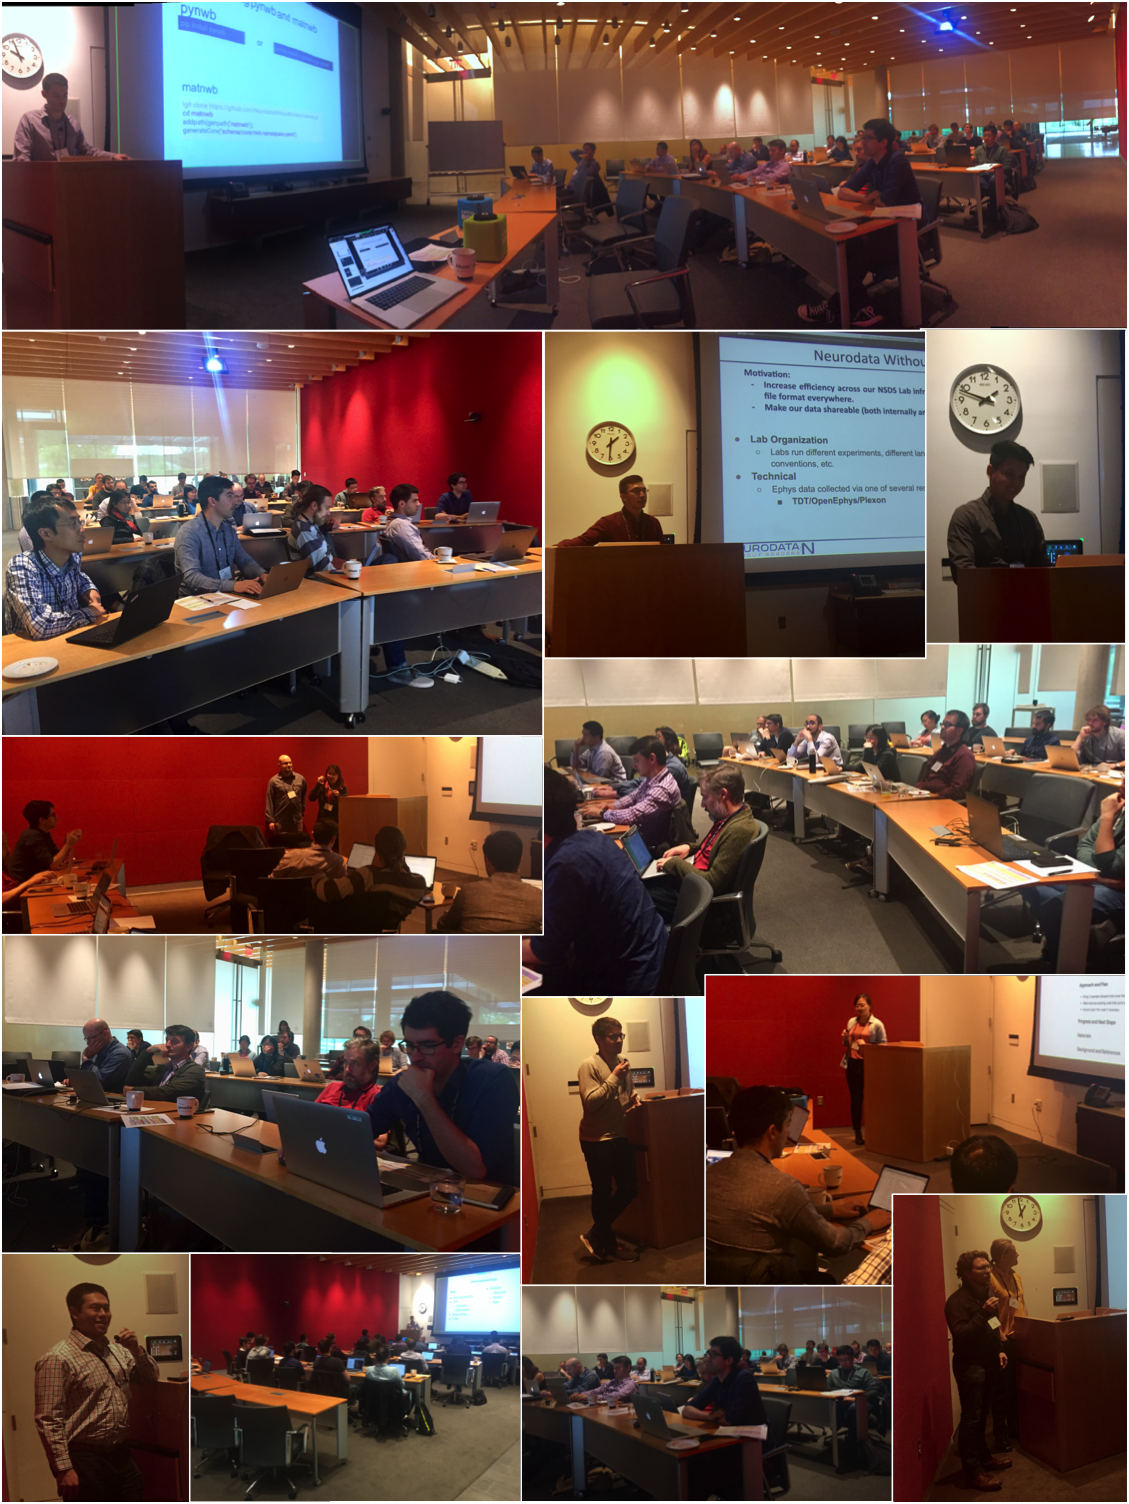
\includegraphics[width=\textwidth]{figures/photos_day1_main_room.png}
\caption{NWB:N User Days, Day 1 (Synapse Room). \textit{(Photos by Oliver R\"ubel, LBNL)}}
\end{figure*}

\clearpage
\begin{figure*}[h!]
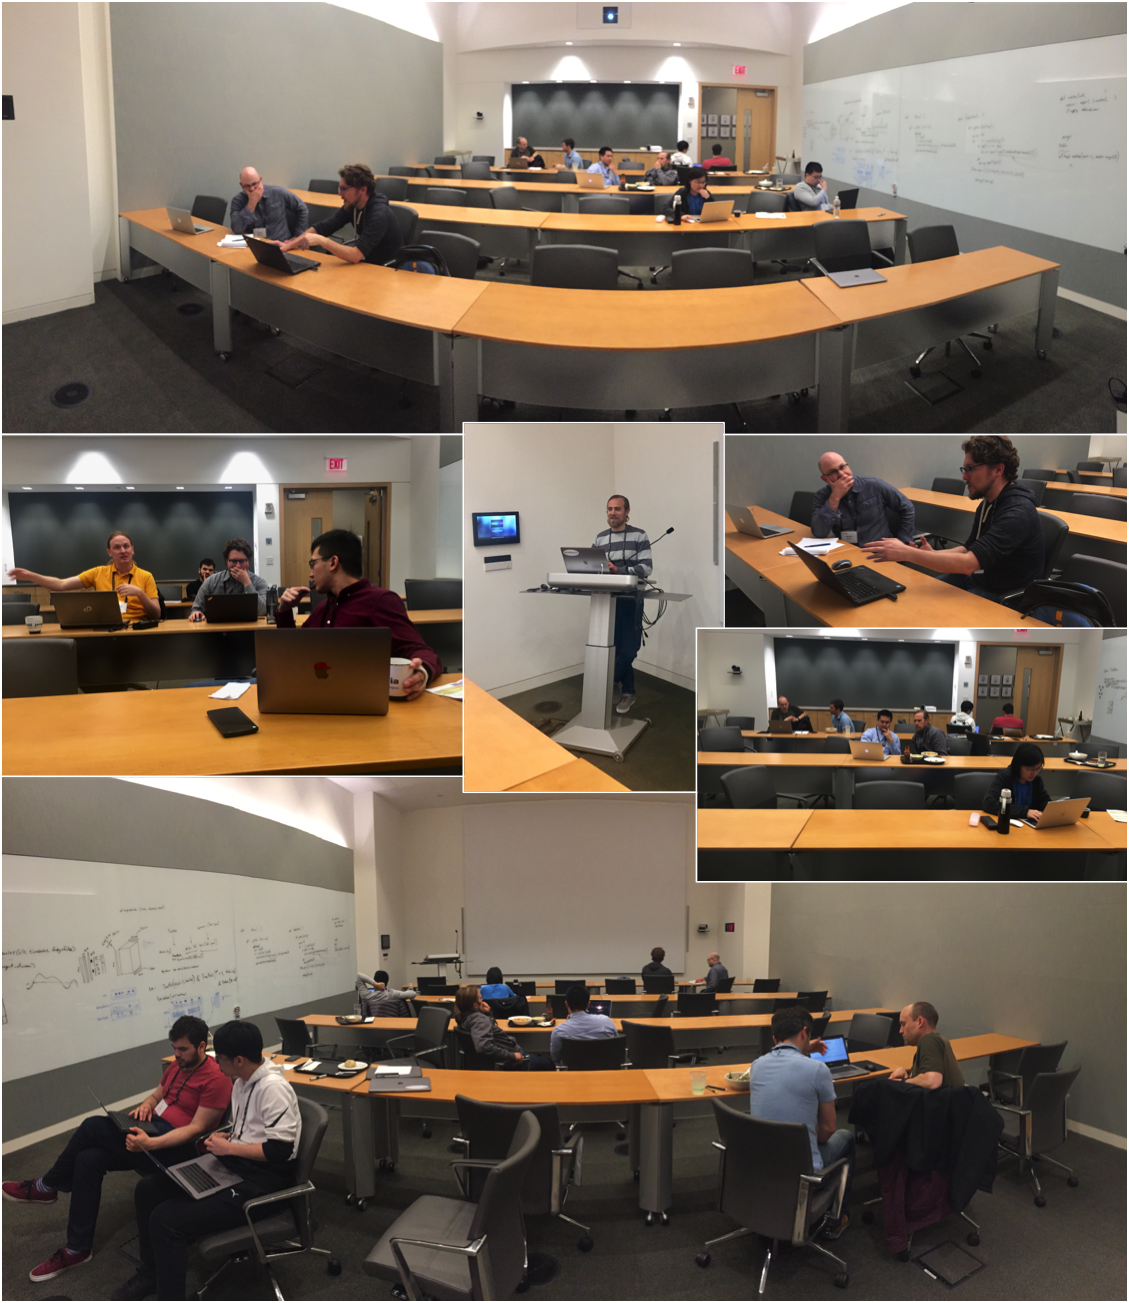
\includegraphics[width=\textwidth]{figures/photos_day1_2_breakout_room.png}
\caption{NWB:N User Days, Day 1-2 (Spectrum Room). \textit{(Photos by Oliver R\"ubel, LBNL)}}
\end{figure*}

\clearpage
\begin{figure*}[h!]
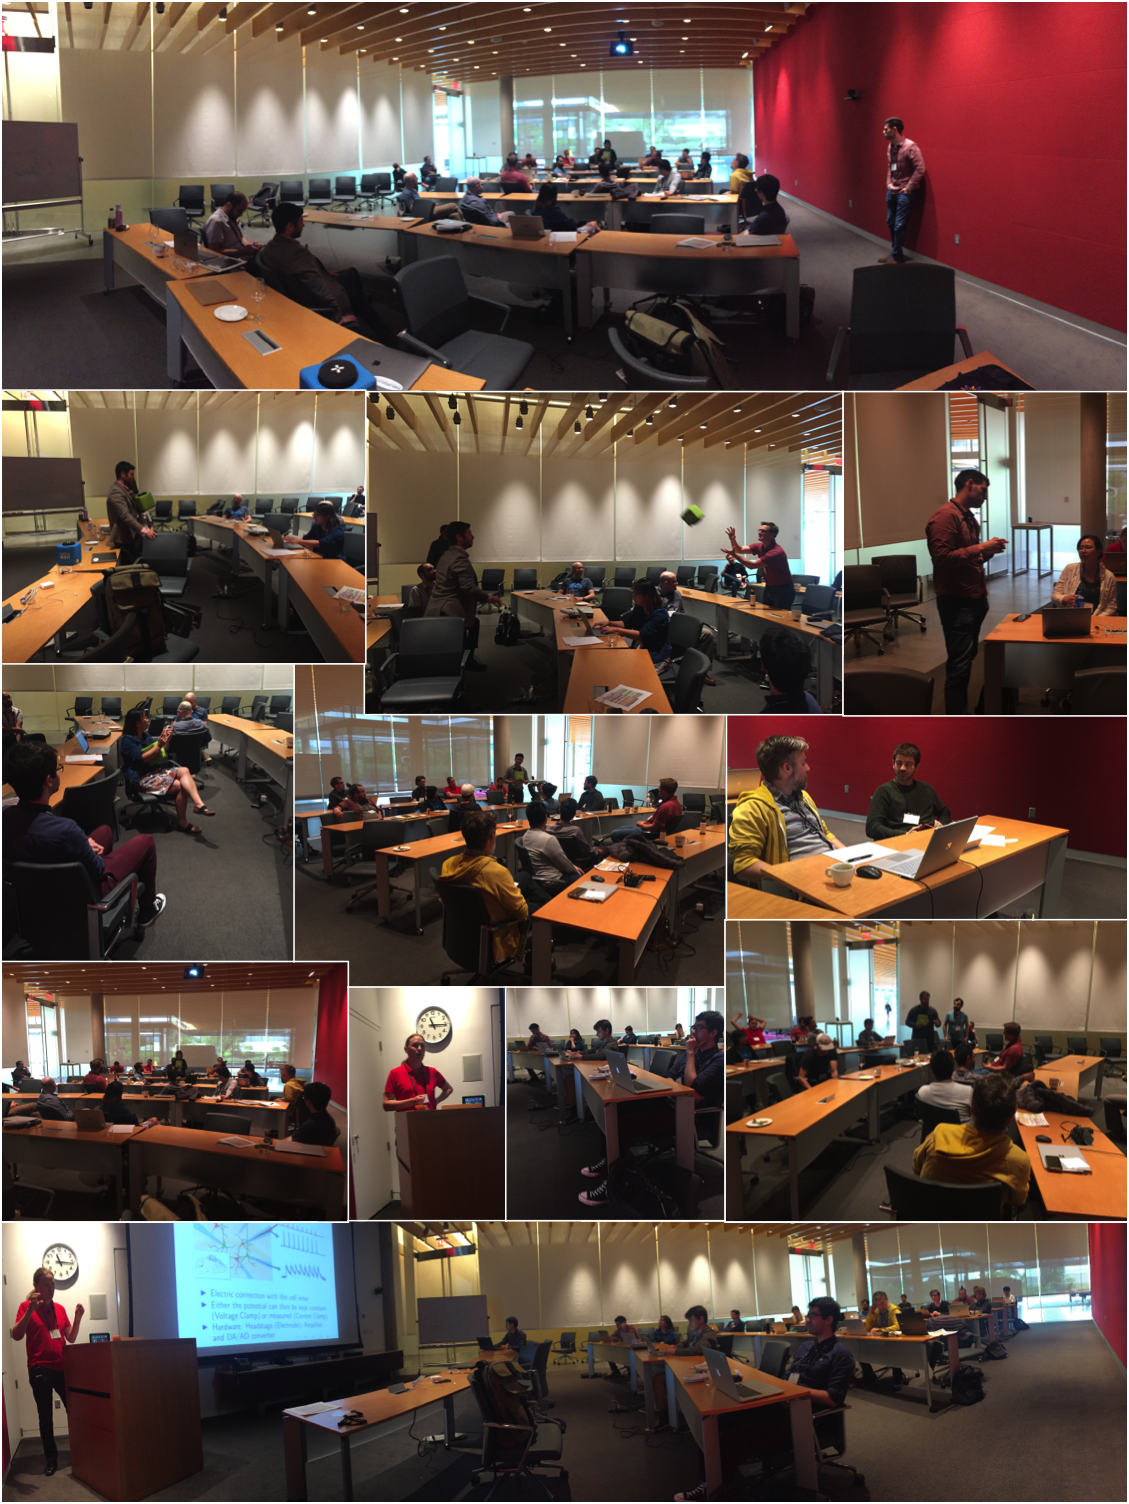
\includegraphics[width=\textwidth]{figures/photos_day2_main_room.png}
\caption{NWB:N User Days, Day 2  (Synapse Room). \textit{(Photos by Oliver R\"ubel, LBNL)}}
\end{figure*}

\clearpage
\begin{figure*}[h!]
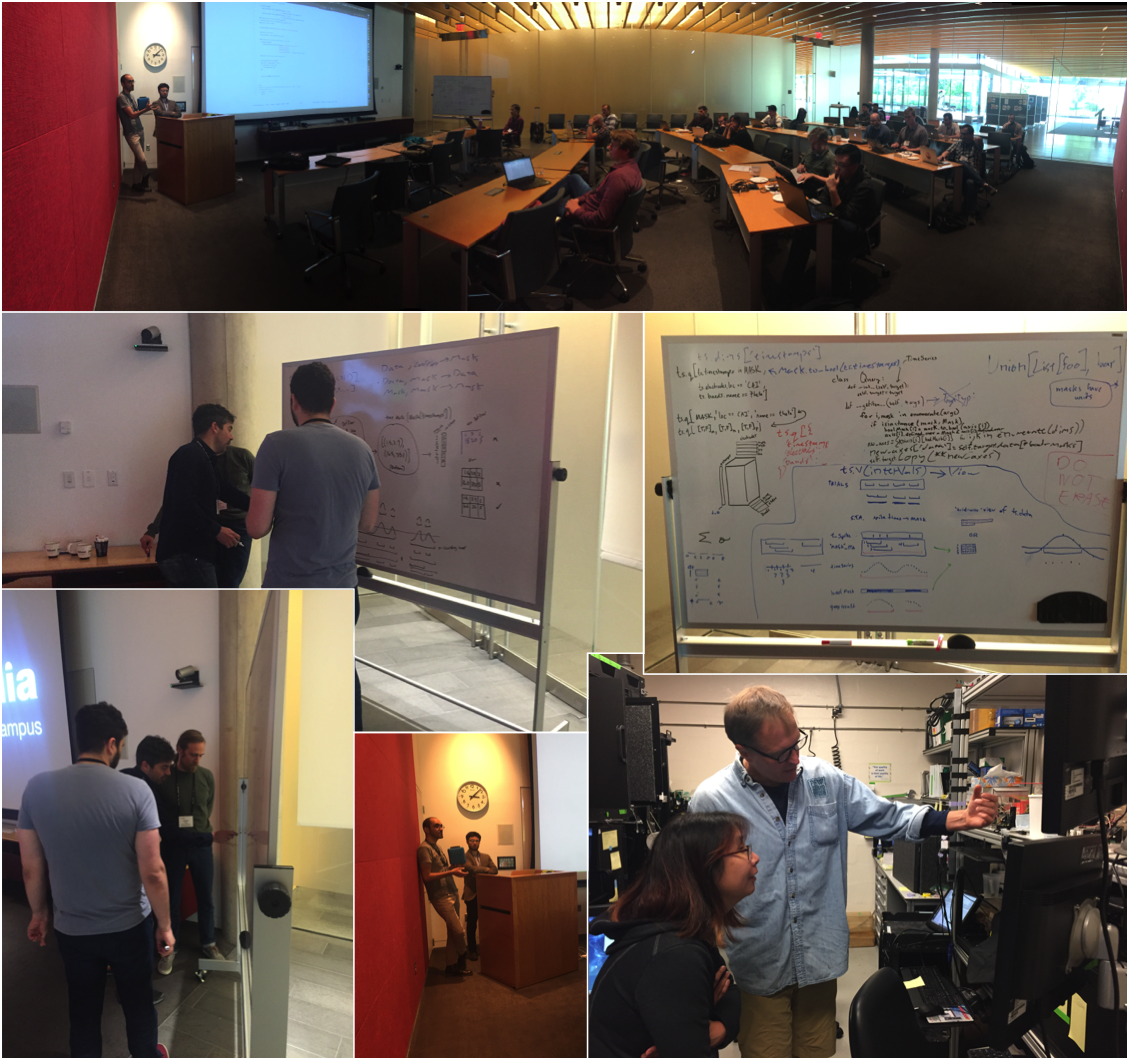
\includegraphics[width=\textwidth]{figures/photos_day3_4_developer_days.png}
\caption{NWB:N Developer Days, Day 3 and 4. \textit{(Photos by Oliver R\"ubel, LBNL)}}
\end{figure*}

\clearpage
\section*{Acknowledgements}
\label{sec:ack}
\addcontentsline{toc}{section}{\nameref{sec:ack}}

We would like to thank Andrew Tritt, Nathan Clack, Lawrence Niu,
Michael Grauer, Ryan Ly, Thomas Braun, Tom Davidson,
Thinh Nguyen, and Vyassa Baratham, Benjamin Dichter, and Oliver R\"ubel 
for their contributions as presenters and facilitators at the event. 
Special thanks also to  Stephanie Albin (Kavli Foundation) 
for travel support, Janine Stephens (HHMI Janelia) for onsite
logistic support, and Matt Staley (HHMI Janelia) for AV support
and photography. We would like to thank all the participants 
for the great enthusiasm and commitment and for making the 
hackathon a great success! We thank the Kavli foundation and
HHMI Janelia for financial support of the hackathon. 


\section*{Disclaimer}
\label{sec:disc}
\addcontentsline{toc}{section}{\nameref{sec:disc}}


This document and related content were prepared as an account of or to expedite 
work sponsored at least in part by the United States Government. While we strive
to provide correct information, neither the United States Government nor any 
agency thereof, nor The Regents of the University of California, nor any of their 
employees, makes any warranty, express or implied, or assumes any legal responsibility
for the accuracy, completeness, or usefulness of any information, apparatus, product,
or process disclosed, or represents that its use would not infringe privately owned rights.

Reference herein to any specific commercial product, process, or service by its 
trade name, trademark, manufacturer, or otherwise, does not necessarily constitute
or imply its endorsement, recommendation, or favoring by the United States Government
or any agency thereof, or The Regents of the University of California. Use of the 
Laboratory or University’s name for endorsements is prohibited.

The views and opinions of authors expressed herein do not necessarily state or reflect 
those of the United States Government or any agency thereof or The Regents of the 
University of California. Neither Berkeley Lab nor its employees are agents of the US Government.

Links to external pages and documents included in the documents do not constitute
an endorsement of the content or company and we are not responsible for the 
content of such links.

\begin{figure}[b!]
\vspace{1cm}
\centering

\includegraphics[width=0.4\textwidth]{figures/nwb_n_logo.png} \\
\href{https://neurodatawithoutborders.github.io/}{https://neurodatawithoutborders.github.io/}
\end{figure}

\end{document}
